% Options for packages loaded elsewhere
% Options for packages loaded elsewhere
\PassOptionsToPackage{unicode}{hyperref}
\PassOptionsToPackage{hyphens}{url}
%
\documentclass[
  12pt,
  letterpaper,
]{scrbook}
\usepackage{xcolor}
\usepackage{amsmath,amssymb}
\setcounter{secnumdepth}{5}
\usepackage{iftex}
\ifPDFTeX
  \usepackage[T1]{fontenc}
  \usepackage[utf8]{inputenc}
  \usepackage{textcomp} % provide euro and other symbols
\else % if luatex or xetex
  \usepackage{unicode-math} % this also loads fontspec
  \defaultfontfeatures{Scale=MatchLowercase}
  \defaultfontfeatures[\rmfamily]{Ligatures=TeX,Scale=1}
\fi
\usepackage{lmodern}
\ifPDFTeX\else
  % xetex/luatex font selection
  \setmainfont[]{Times New Roman}
\fi
% Use upquote if available, for straight quotes in verbatim environments
\IfFileExists{upquote.sty}{\usepackage{upquote}}{}
\IfFileExists{microtype.sty}{% use microtype if available
  \usepackage[]{microtype}
  \UseMicrotypeSet[protrusion]{basicmath} % disable protrusion for tt fonts
}{}
\makeatletter
\@ifundefined{KOMAClassName}{% if non-KOMA class
  \IfFileExists{parskip.sty}{%
    \usepackage{parskip}
  }{% else
    \setlength{\parindent}{0pt}
    \setlength{\parskip}{6pt plus 2pt minus 1pt}}
}{% if KOMA class
  \KOMAoptions{parskip=half}}
\makeatother
% Make \paragraph and \subparagraph free-standing
\makeatletter
\ifx\paragraph\undefined\else
  \let\oldparagraph\paragraph
  \renewcommand{\paragraph}{
    \@ifstar
      \xxxParagraphStar
      \xxxParagraphNoStar
  }
  \newcommand{\xxxParagraphStar}[1]{\oldparagraph*{#1}\mbox{}}
  \newcommand{\xxxParagraphNoStar}[1]{\oldparagraph{#1}\mbox{}}
\fi
\ifx\subparagraph\undefined\else
  \let\oldsubparagraph\subparagraph
  \renewcommand{\subparagraph}{
    \@ifstar
      \xxxSubParagraphStar
      \xxxSubParagraphNoStar
  }
  \newcommand{\xxxSubParagraphStar}[1]{\oldsubparagraph*{#1}\mbox{}}
  \newcommand{\xxxSubParagraphNoStar}[1]{\oldsubparagraph{#1}\mbox{}}
\fi
\makeatother

\usepackage{color}
\usepackage{fancyvrb}
\newcommand{\VerbBar}{|}
\newcommand{\VERB}{\Verb[commandchars=\\\{\}]}
\DefineVerbatimEnvironment{Highlighting}{Verbatim}{commandchars=\\\{\}}
% Add ',fontsize=\small' for more characters per line
\usepackage{framed}
\definecolor{shadecolor}{RGB}{241,243,245}
\newenvironment{Shaded}{\begin{snugshade}}{\end{snugshade}}
\newcommand{\AlertTok}[1]{\textcolor[rgb]{0.68,0.00,0.00}{#1}}
\newcommand{\AnnotationTok}[1]{\textcolor[rgb]{0.37,0.37,0.37}{#1}}
\newcommand{\AttributeTok}[1]{\textcolor[rgb]{0.40,0.45,0.13}{#1}}
\newcommand{\BaseNTok}[1]{\textcolor[rgb]{0.68,0.00,0.00}{#1}}
\newcommand{\BuiltInTok}[1]{\textcolor[rgb]{0.00,0.23,0.31}{#1}}
\newcommand{\CharTok}[1]{\textcolor[rgb]{0.13,0.47,0.30}{#1}}
\newcommand{\CommentTok}[1]{\textcolor[rgb]{0.37,0.37,0.37}{#1}}
\newcommand{\CommentVarTok}[1]{\textcolor[rgb]{0.37,0.37,0.37}{\textit{#1}}}
\newcommand{\ConstantTok}[1]{\textcolor[rgb]{0.56,0.35,0.01}{#1}}
\newcommand{\ControlFlowTok}[1]{\textcolor[rgb]{0.00,0.23,0.31}{\textbf{#1}}}
\newcommand{\DataTypeTok}[1]{\textcolor[rgb]{0.68,0.00,0.00}{#1}}
\newcommand{\DecValTok}[1]{\textcolor[rgb]{0.68,0.00,0.00}{#1}}
\newcommand{\DocumentationTok}[1]{\textcolor[rgb]{0.37,0.37,0.37}{\textit{#1}}}
\newcommand{\ErrorTok}[1]{\textcolor[rgb]{0.68,0.00,0.00}{#1}}
\newcommand{\ExtensionTok}[1]{\textcolor[rgb]{0.00,0.23,0.31}{#1}}
\newcommand{\FloatTok}[1]{\textcolor[rgb]{0.68,0.00,0.00}{#1}}
\newcommand{\FunctionTok}[1]{\textcolor[rgb]{0.28,0.35,0.67}{#1}}
\newcommand{\ImportTok}[1]{\textcolor[rgb]{0.00,0.46,0.62}{#1}}
\newcommand{\InformationTok}[1]{\textcolor[rgb]{0.37,0.37,0.37}{#1}}
\newcommand{\KeywordTok}[1]{\textcolor[rgb]{0.00,0.23,0.31}{\textbf{#1}}}
\newcommand{\NormalTok}[1]{\textcolor[rgb]{0.00,0.23,0.31}{#1}}
\newcommand{\OperatorTok}[1]{\textcolor[rgb]{0.37,0.37,0.37}{#1}}
\newcommand{\OtherTok}[1]{\textcolor[rgb]{0.00,0.23,0.31}{#1}}
\newcommand{\PreprocessorTok}[1]{\textcolor[rgb]{0.68,0.00,0.00}{#1}}
\newcommand{\RegionMarkerTok}[1]{\textcolor[rgb]{0.00,0.23,0.31}{#1}}
\newcommand{\SpecialCharTok}[1]{\textcolor[rgb]{0.37,0.37,0.37}{#1}}
\newcommand{\SpecialStringTok}[1]{\textcolor[rgb]{0.13,0.47,0.30}{#1}}
\newcommand{\StringTok}[1]{\textcolor[rgb]{0.13,0.47,0.30}{#1}}
\newcommand{\VariableTok}[1]{\textcolor[rgb]{0.07,0.07,0.07}{#1}}
\newcommand{\VerbatimStringTok}[1]{\textcolor[rgb]{0.13,0.47,0.30}{#1}}
\newcommand{\WarningTok}[1]{\textcolor[rgb]{0.37,0.37,0.37}{\textit{#1}}}

\usepackage{longtable,booktabs,array}
\usepackage{calc} % for calculating minipage widths
% Correct order of tables after \paragraph or \subparagraph
\usepackage{etoolbox}
\makeatletter
\patchcmd\longtable{\par}{\if@noskipsec\mbox{}\fi\par}{}{}
\makeatother
% Allow footnotes in longtable head/foot
\IfFileExists{footnotehyper.sty}{\usepackage{footnotehyper}}{\usepackage{footnote}}
\makesavenoteenv{longtable}
\usepackage{graphicx}
\makeatletter
\newsavebox\pandoc@box
\newcommand*\pandocbounded[1]{% scales image to fit in text height/width
  \sbox\pandoc@box{#1}%
  \Gscale@div\@tempa{\textheight}{\dimexpr\ht\pandoc@box+\dp\pandoc@box\relax}%
  \Gscale@div\@tempb{\linewidth}{\wd\pandoc@box}%
  \ifdim\@tempb\p@<\@tempa\p@\let\@tempa\@tempb\fi% select the smaller of both
  \ifdim\@tempa\p@<\p@\scalebox{\@tempa}{\usebox\pandoc@box}%
  \else\usebox{\pandoc@box}%
  \fi%
}
% Set default figure placement to htbp
\def\fps@figure{htbp}
\makeatother


% definitions for citeproc citations
\NewDocumentCommand\citeproctext{}{}
\NewDocumentCommand\citeproc{mm}{%
  \begingroup\def\citeproctext{#2}\cite{#1}\endgroup}
\makeatletter
 % allow citations to break across lines
 \let\@cite@ofmt\@firstofone
 % avoid brackets around text for \cite:
 \def\@biblabel#1{}
 \def\@cite#1#2{{#1\if@tempswa , #2\fi}}
\makeatother
\newlength{\cslhangindent}
\setlength{\cslhangindent}{1.5em}
\newlength{\csllabelwidth}
\setlength{\csllabelwidth}{3em}
\newenvironment{CSLReferences}[2] % #1 hanging-indent, #2 entry-spacing
 {\begin{list}{}{%
  \setlength{\itemindent}{0pt}
  \setlength{\leftmargin}{0pt}
  \setlength{\parsep}{0pt}
  % turn on hanging indent if param 1 is 1
  \ifodd #1
   \setlength{\leftmargin}{\cslhangindent}
   \setlength{\itemindent}{-1\cslhangindent}
  \fi
  % set entry spacing
  \setlength{\itemsep}{#2\baselineskip}}}
 {\end{list}}
\usepackage{calc}
\newcommand{\CSLBlock}[1]{\hfill\break\parbox[t]{\linewidth}{\strut\ignorespaces#1\strut}}
\newcommand{\CSLLeftMargin}[1]{\parbox[t]{\csllabelwidth}{\strut#1\strut}}
\newcommand{\CSLRightInline}[1]{\parbox[t]{\linewidth - \csllabelwidth}{\strut#1\strut}}
\newcommand{\CSLIndent}[1]{\hspace{\cslhangindent}#1}



\setlength{\emergencystretch}{3em} % prevent overfull lines

\providecommand{\tightlist}{%
  \setlength{\itemsep}{0pt}\setlength{\parskip}{0pt}}



 


\usepackage{tcolorbox}
\usepackage{amssymb}
\usepackage{yfonts}
\usepackage{bm}


\newtcolorbox{greybox}{
  colback=white,
  colframe=blue,
  coltext=black,
  boxsep=5pt,
  arc=4pt}
  
\newcommand{\sectionbreak}{\clearpage}

 
\newcommand{\ds}[4]{\sum_{{#1}=1}^{#3}\sum_{{#2}=1}^{#4}}
\newcommand{\us}[3]{\mathop{\sum\sum}_{1\leq{#2}<{#1}\leq{#3}}}

\newcommand{\ol}[1]{\overline{#1}}
\newcommand{\ul}[1]{\underline{#1}}

\newcommand{\amin}[1]{\mathop{\text{argmin}}_{#1}}
\newcommand{\amax}[1]{\mathop{\text{argmax}}_{#1}}

\newcommand{\ci}{\perp\!\!\!\perp}

\newcommand{\mc}[1]{\mathcal{#1}}
\newcommand{\mb}[1]{\mathbb{#1}}
\newcommand{\mf}[1]{\mathfrak{#1}}

\newcommand{\eps}{\epsilon}
\newcommand{\lbd}{\lambda}
\newcommand{\alp}{\alpha}
\newcommand{\df}{=:}
\newcommand{\am}[1]{\mathop{\text{argmin}}_{#1}}
\newcommand{\ls}[2]{\mathop{\sum\sum}_{#1}^{#2}}
\newcommand{\ijs}{\mathop{\sum\sum}_{1\leq i<j\leq n}}
\newcommand{\jis}{\mathop{\sum\sum}_{1\leq j<i\leq n}}
\newcommand{\sij}{\sum_{i=1}^n\sum_{j=1}^n}
	
\makeatletter
\@ifpackageloaded{bookmark}{}{\usepackage{bookmark}}
\makeatother
\makeatletter
\@ifpackageloaded{caption}{}{\usepackage{caption}}
\AtBeginDocument{%
\ifdefined\contentsname
  \renewcommand*\contentsname{Table of contents}
\else
  \newcommand\contentsname{Table of contents}
\fi
\ifdefined\listfigurename
  \renewcommand*\listfigurename{List of Figures}
\else
  \newcommand\listfigurename{List of Figures}
\fi
\ifdefined\listtablename
  \renewcommand*\listtablename{List of Tables}
\else
  \newcommand\listtablename{List of Tables}
\fi
\ifdefined\figurename
  \renewcommand*\figurename{Figure}
\else
  \newcommand\figurename{Figure}
\fi
\ifdefined\tablename
  \renewcommand*\tablename{Table}
\else
  \newcommand\tablename{Table}
\fi
}
\@ifpackageloaded{float}{}{\usepackage{float}}
\floatstyle{ruled}
\@ifundefined{c@chapter}{\newfloat{codelisting}{h}{lop}}{\newfloat{codelisting}{h}{lop}[chapter]}
\floatname{codelisting}{Listing}
\newcommand*\listoflistings{\listof{codelisting}{List of Listings}}
\makeatother
\makeatletter
\makeatother
\makeatletter
\@ifpackageloaded{caption}{}{\usepackage{caption}}
\@ifpackageloaded{subcaption}{}{\usepackage{subcaption}}
\makeatother
\usepackage{bookmark}
\IfFileExists{xurl.sty}{\usepackage{xurl}}{} % add URL line breaks if available
\urlstyle{same}
\hypersetup{
  pdftitle={Gifi Analysis of Multivariate Data},
  pdfauthor={Jan de Leeuw},
  hidelinks,
  pdfcreator={LaTeX via pandoc}}


\title{Gifi Analysis of Multivariate Data}
\author{Jan de Leeuw}
\date{May 5, 2025}
\begin{document}
\frontmatter
\maketitle

\renewcommand*\contentsname{Table of contents}
{
\setcounter{tocdepth}{2}
\tableofcontents
}

\mainmatter
\bookmarksetup{startatroot}

\chapter*{Preface}\label{preface}
\addcontentsline{toc}{chapter}{Preface}

\markboth{Preface}{Preface}

In 1980 members of the Department of Data Theory at the University of
Leiden taught a post-doctoral course in Nonlinear Multivariate Analysis.
The course content was sort-of-published, in Dutch, as Gifi
(\citeproc{ref-gifi_B_80}{1980}). The course was repeated in 1981, and
this time the sort-of-published version (Gifi
(\citeproc{ref-gifi_B_81}{1981})) was in English.

The preface gives some details about the author.

\begin{quote}
The text is the joint product of the members of the Department of Data
Theory of the Faculty of Social Sciences, University of Leiden. `Albert
Gifi' is their `nom de plume'. The portrait, however, of Albert Gifi
shown here, is that of the real Albert Gifi to whose memory this book is
dedicated, as a far too late recompense for his loyalty and devotion,
during so any years, to the Cause he served.
\end{quote}

Roughly ten years later a revised version of these course notes came out
as an actual book in the \emph{Wiley Series in Probabilty and
Mathematical Statistics} (Gifi (\citeproc{ref-gifi_B_90}{1990})). This
despite the fact that the contents of the book had very little to do
with either probability or mathematical statistics. The book is
organized around a series of computer programs for correspondence
analysis, principal component analysis, and canonical analysis. The
programs, written in FORTRAN, are called HOMALS, PRINCALS, PRIMALS,
CRIMINALS, CANALS, OVERALS because they combine classical linear
multivariate analysis with optimal transformation of the variables,
using alternating least squares (or ALS). It serves, to some extent, as
a manual for the programs, but it also discusses the properties of the
techniques implemented in the programs, and it presents many detailed
applications of these techniques.

Reviewers generally had some difficulties separating the wheat from the
chaff.

\begin{quote}
As the spirit of Albert Gifi has faded away, so has his whimsical
approach to publishing, and his latest book is an idiosyncratic account
of multivariate methods developed by the Leiden group during the 1970s.
The names of their computer programs are distinguished by the ending
\textasciitilde ALS, thus we have OVERALS, PRINCALS, HOMALS, CANALS,
MORALS, MANOVALS, CRIMINALS, PARTALS and PATHALS. Perhaps if you have a
warped mind like this reviewer, you will turn rapidly to CRIMINALS. What
can it be ? Surely it must give some illicit view of the truth about the
world, a vision of the underworld of multivariate analysis ? Alas no !
It turns out only to be a synonym of Canonical Variate Analysis,
sometimes known as Multiple Discriminant Analysis. Likewise HOMALS turns
out to be Reciprocal Averaging, otherwise known as Correspondence
Analysis. (Hill (\citeproc{ref-hill_90}{1990}))
\end{quote}

This ambiguity and confusion are not too surprising. The Gifi book was a
summary of the work of a large number of people, over a period of almost
20 years. Nevertheless, and perhaps because of this, it is somewhat of a
\emph{camel}, which we define for our purposes as a \emph{horse designed
by a committee}. Different chapters had different authors, and the
common ideas behind the various techniques were not always clearly
explained.

\begin{quote}
In Gifi's MVA the criterion called ``meet'' loss plays a central role.
Although the adoption of this criterion is one of the most important
contributions of Gifi, the book would have been much more readable if
this criterion had been introduced right at the outset and was followed
throughout the rest of the book. (Takane
(\citeproc{ref-takane_92}{1992}))
\end{quote}

Nevertheless there is much original material in Gifi
(\citeproc{ref-gifi_B_90}{1990}), and the book has early applications of
alternating least squares, majorization, coordinate descent, the delta
method, and the bootstrap. And it emphasizes throughout the idea that
statistics is about techniques, not about models. But, yes, the
organization leaves much to be desired. An on demand printing of the
first and only edition is now available on Amazon for \$ 492 -- although
of course used versions go for much less.

The book was published by a prestiguous publisher in a prestiguous
series, but it is fair to say it never really caught on. It is not hard
to understand why. The content, and the style, are unfamiliar to
statisticians and mathematicians. There is no inference, no probability,
and very little rigor. The content is in multivariate data analysis,
which would be most at home these days, if anywhere, in a computer
science department. The Gifi group did not have the resources of, say,
Benzécri in France or Hayashi in Japan. The members were mostly active
in psychometrics, a small and insular field, and they were from The
Netherlands, a small country prone to overestimate its importance
(Marvell (\citeproc{ref-marvell_53}{1653})). They also did not have the
evangelical zeal necessary for creating and sustaining a large impact.

There have been some other major publication events in the Gifi saga.
Around the same time as the Wiley book there was the publication of SPSS
(\citeproc{ref-spss_89}{1989}). Starting in the late seventies the Gifi
FORTRAN programs had been embedded in the SPSS system. The \emph{SPSS
Categories} manual was updated many times, in fact every time SPSS or
IBM SPSS had a new release. Over the years other programs produced by
the Department of Data Theory were added. A recent version is, for
example, Meulman and Heiser (\citeproc{ref-meulman_heiser_12}{2012}),
corresponding to IBM SPSS 21. It acknowledges the contributions of some
of the members of the Gifi team -- but in IBM
(\citeproc{ref-ibm_15}{2015}), the version for IBM SPSS 23, these
acknowledgements and the names of the authors have disappeared. Sic
transit gloria mundi.

Michailidis and De Leeuw (\citeproc{ref-michailidis_deleeuw_A_98}{1998})
made an attempt to make the Gifi material somewhat more accessible by
publishing a review article in a widely read mainstream statistical
journal. Another such attempt is De Leeuw and Mair
(\citeproc{ref-deleeuw_mair_A_09a}{2009}), in which the homals package
for R is introduced. The homals package is basically a single monolithic
R function that can do everything the Gifi programs can do, and then
some. In both cases, however, the problem remained that the techniques,
and the software, were too convoluted and too different from what both
statisticians and users were accustomed to.

Van der Heijden and Van Buuren
(\citeproc{ref-vanderheijden_vanbuuren_16}{1916}) give an excellent,
though somewhat wistful, historic overview of the Gifi project. It is
too early for eulogies, however, and we refuse to give up. This book is
yet another reorganization of the Gifi material, with many extensions.
We take Yoshio Takane's advice seriously, and we organize both the
theory and the algorithms around what is called ``meet-loss'' in Gifi.
In our software we separate the basic computational engine from its
various applications that define the techniques of \emph{Multivariate
Analysis with Optimal Scaling (MVAOS)}. Hiding the core makes it
possible to make the programs behave in much the same way as traditional
MVA programs. The software is written in R
((\citeproc{ref-r_core_team_16}{\textbf{r\_core\_team\_16?}})), with
some parts of the computational engine written in C.

The book itself is written in Rmarkdown, using bookdown (Xie
(\citeproc{ref-xie_16}{2016})) and knitr (Xie
(\citeproc{ref-xie_15}{2015})) to embed the computations and graphics,
and to produce html and pdf versions that are completely reproducible.
The book and all the files that go with it are in the public domain.

We would like to acknowledge those who have made substantial
contributions to the Gifi project (and its immediate ancestors and
offspring) over the years. Some of them are lost in the mists of time,
some of them are no longer on this earth. They are, in alphabetical
order, Bert Bettonvil, Jason Bond, Catrien Bijleveld, Frank Busing,
Jacques Commandeur, Henny Coolen, Steef de Bie, Jan de Leeuw, John
Gower, Patrick Groenen, Chris Haveman, Willem Heiser, Abby Israels, Judy
Knip, Jan Koster, Pieter Kroonenberg, Patrick Mair, Adriaan Meester,
Jacqueline Meulman, George Michailidis, Peter Neufeglise, Dré Nierop,
Ineke Stoop, Yoshio Takane, Stef van Buuren, John van de Geer, Gerda van
den Berg, Eeke van der Burg, Peter van der Heijden, Anita van der Kooij,
Ivo van der Lans, Rien van der Leeden, Jan van Rijckevorsel, Renée
Verdegaal, Peter Verboon, Susañña Verdel, and Forrest Young.

\bookmarksetup{startatroot}

\chapter{Introduction}\label{introduction}

One way of looking at \emph{Multivariate Analysis with Optimal Scaling},
or \emph{MVAOS}, is as an extension of classical linear multivariate
analysis to variables that are binary, ordered, or even unordered
categorical. In R terminology, classical MVA techniques can thus be
applied if some or all of the variables in the dataframe are
\emph{factors}. Categorical variables are \emph{quantified} and
numerical variables are \emph{transformed} to optimize the linear or
bilinear least squares fit.

Least squares and eigenvalue methods for quantifying multivariate
qualitative data were first introduced by Guttman
(\citeproc{ref-guttman_41}{1941}), although there were some bivariate
predecessors in the work of Pearson, Fisher, Maung, and Hirschfeld (see
De Leeuw (\citeproc{ref-deleeuw_A_83b}{1983}) or Gower
(\citeproc{ref-gower_90}{1990}) for a historical overview). In this
earlier work the emphasis was often on optimizing quadratic forms, or
ratios of quadratic forms, and not so much on least squares, distance
geometry, and graphical representations such as \emph{biplots} (Gower
and Hand (\citeproc{ref-gower_hand_96}{1996}), Gower, Le Roux, and
Gardner-Lubbe (\citeproc{ref-gower_leroux_gardnerlubbe_15}{2015}),
Gower, Le Roux, and Gardner-Lubbe
(\citeproc{ref-gower_leroux_gardnerlubbe_16}{2016})). They were taken up
by, among others, De Leeuw (\citeproc{ref-deleeuw_R_68e}{1968a}), by
Benzécri and his students in France (see Cordier
(\citeproc{ref-cordier_65}{1965})), and by Hayashi and his students in
Japan (see Tanaka (\citeproc{ref-tanaka_79}{1979})). Early applications
can be found in ecology, following an influential paper by Hill
(\citeproc{ref-hill_74}{1974}). With increasing emphasis on software the
role of graphical representations has increased and continues to
increase.

In De Leeuw (\citeproc{ref-deleeuw_B_74}{1974}) a first attempt was made
to unify most classical descriptive multivariate techniques using a
single least squares loss function and a corresponding \emph{alternating
least squares (ALS)} optimization method. His work then bifurcated to
the \emph{ALSOS project}, with Young and Takane at the University of
North Carolina Chapell Hill, and the \emph{Gifi project}, at the
Department of Data Theory of Leiden University.

The ALSOS project was started in 1973-1974, when De Leeuw was visiting
Bell Telephone Labs in Murray Hill. ALSOS stands for Alternating Least
Squares with Optimal Scaling. The ALS part of the name was provided by
De Leeuw (\citeproc{ref-deleeuw_R_68d}{1968b}) and the OS part by Bock
(\citeproc{ref-bock_60}{1960}). At early meetings of the Psychometric
Society some members were offended by our use of ``Optimal Scaling'',
because they took it to imply that their methods of scaling were
supposedly inferior to ours. But the ``optimal'' merely refers to
optimality in the context of a specific least squares loss function.

Young, De Leeuw, and Takane applied the basic ALS and OS methodology to
conjoint analysis, regression, principal component analysis,
multidimensional scaling, and factor analysis, producing computer
programs (and SAS modules) for each of the techniques. An overview of
the project, basically at the end of its lifetime, is in Young, De
Leeuw, and Takane (\citeproc{ref-young_deleeuw_takane_C_80}{1980}) and
Young (\citeproc{ref-young_81}{1981}).

The ALSOS project was clearly inspired by the path-breaking work of
Kruskal (\citeproc{ref-kruskal_64a}{1964a}) and Kruskal
(\citeproc{ref-kruskal_64b}{1964b}), who designed a general way to turn
metric multivariate analysis techniques into non-metric ones. In fact,
Kruskal applied the basic methodology developed for multidimensional
scaling to linear models in Kruskal (\citeproc{ref-kruskal_65}{1965}),
and to principal component analysis in Kruskal and Shepard
(\citeproc{ref-kruskal_shepard_74}{1974}) (which was actually written
around 1965 as well). In parallel developments closely related nonmetric
methods were developed by Roskam (\citeproc{ref-roskam_68}{1968}) and by
Guttman and Lingoes (see Lingoes (\citeproc{ref-lingoes_73}{1973})).

The Gifi project took its inspiration from Kruskal, but perhaps even
more from Guttman (\citeproc{ref-guttman_41}{1941}) (and to a lesser
extent from the optimal scaling work of Fisher, see Gower
(\citeproc{ref-gower_90}{1990})). Guttman's quantification method, which
later became known as \emph{multiple correspondence analysis}, was
merged with linear and nonlinear principal component analysis in the
HOMALS/PRINCALS techniques and programs (De Leeuw and Rijckevorsel
(\citeproc{ref-deleeuw_vanrijckevorsel_C_80}{1980})). The MVAOS loss
function that was chosen ultimately, for example in the work of Burg, De
Leeuw, and Verdegaal
(\citeproc{ref-vanderburg_deleeuw_verdegaal_A_88}{1988}), had been used
earlier by Carroll (\citeproc{ref-carroll_68}{1968}) in multi-set
canonical correlation analysis of numerical variables.

A project similar to ALSOS/Gifi was ACE, short for \emph{Alternating
Conditional Expectations}. The ACE method for regression was introduced
by Breiman and Friedman (\citeproc{ref-breiman_friedman_85}{1985}) and
the ACE method for principal component analysis by Koyak
(\citeproc{ref-koyak_87}{1987}). Both techniques use the same ALS block
relaxation methods, but instead of projecting on a cone or subspace of
possible transformation, they apply a smoother (typically Friedman's
supersmoother) to find the optimal transformation. This implies that the
method is intended primarily for continuous variables, and that the
convergence properties of the ACE algorithm are more complicated than
those of a proper ALS algorithms.

An even more closely related project, by Winsberg and Ramsay, uses the
cone of I-splines (integrated B-splines) to define the optimal
transformations. The technique for linear models is in Winsberg and
Ramsay (\citeproc{ref-winsberg_ramsay_80}{1980}) and the one for
principal component analysis in Winsberg and Ramsay
(\citeproc{ref-winsberg_ramsay_83}{1983}). Again, the emphasis on
monotonic splines indicates that continuous variables play a larger role
than in the ALSOS or Gifi system.

So generally there have been a number of projects over the last 50 years
that differ in detail, but apply basically the same methodology
(alternating least squares and optimal scaling) to generalize classical
MVA techniques. Some of them emphasize transformation of continuous
variables, some emphasize quantification of discrete variables. Some
emphasize monotonicity, some smoothness. Usually these projects include
techniques for regression and principal component analysis, but in the
case of Gifi the various forms of correspondence analysis and canonical
analysis are also included.

\section{Beyond Gifi}\label{beyond-gifi}

The techniques discussed in Gifi (\citeproc{ref-gifi_B_90}{1990}), and
implemented in the corresponding computer programs, use a particular
least squares loss function and minimize it by alternating least squares
algorithms. All techniques use what Gifi calls \emph{meet loss}, which
is basically the loss function proposed by Carroll
(\citeproc{ref-carroll_68}{1968}) for multiset canonical correlation
analysis. Carroll's work was extended in Gifi by using optimal scaling
to transform or quantify variables coded with indicators, and to use
constraints on the parameters to adapt the basic technique, often called
\emph{homogeneity analysis}, to different classical MVA techniques.

There have been various extensions of the classical Gifi repertoire by
adding techniques that do not readily fit into meet loss. Examples are
path analysis (Coolen and De Leeuw
(\citeproc{ref-coolen_deleeuw_R_87}{1987})), linear dynamic systems
(Bijleveld and De Leeuw (\citeproc{ref-bijleveld_deleeuw_A_91}{1991})),
and factor analysis (De Leeuw (\citeproc{ref-deleeuw_C_04a}{2004})). But
adding these techniques does not really add up to a new framework.

Somewhat more importantly, De Leeuw and Rijckevorsel
(\citeproc{ref-deleeuw_vanrijckevorsel_C_88}{1988}) discuss various ways
to generalize meet loss by using \emph{fuzzy coding}. Transformations
are no longer step functions, and coding can be done with fuzzy
indicators, such as B-spline bases. This makes it easier to deal with
variables that have many ordered categories. Although this is a
substantial generalization the basic framework remains the same.

One of the outgrowths of the Gifi project was the \emph{aspect}
approach, first discussed systematically by De Leeuw
(\citeproc{ref-deleeuw_C_88b}{1988}), and implemented in the R package
\texttt{aspect} by Mair and De Leeuw
(\citeproc{ref-mair_deleeuw_A_10}{2010}). In its original formulation it
uses \emph{majorization} to optimize functions defined on the space of
correlation matrices, where the correlations are computed over
transformed variables, coded by indicators. Thus we optimize aspects of
the correlation matrix over transformations of the variables. The
\texttt{aspect} software was recently updated to allow for B-spline
transformations (De Leeuw (\citeproc{ref-deleeuw_E_15b}{2015a})). Many
different aspects were implemented, based on eigenvalues, determinants,
multiple correlations, and sums of powers of correlation coefficients.
Unformately, aspects defined in terms of canonical correlations, or
generalized canonical correlations, were not covered. Thus the range of
techniques covered by the \texttt{aspect} approach has multiple
regression and principal component analysis in common with the range of
the Gifi system, but is otherwise disjoint from it.

In De Leeuw (\citeproc{ref-deleeuw_C_04a}{2004}) a particular
correlation aspect was singled out that could bridge the gap between the
aspect approach and the Gifi approach, provided \emph{orthoblocks} of
transformations were introduced. This is combined with the notion of
\emph{copies}, introduced in De Leeuw
(\citeproc{ref-deleeuw_C_84c}{1984}), to design a new class of
techniques that encompasses all of Gifi and that brings generalized
canonical correlation analysis in the aspect framework. Thus correlation
aspects, and the majorization algorithms to optimize them, are now a
true generalization of the Gifi system.

*** This is the system we discuss in this book.

\bookmarksetup{startatroot}

\chapter{Coding and Transformations}\label{coding-and-transformations}

\section{Variables and
Multivariables}\label{variables-and-multivariables}

In the multivariate analysis techniques presented in this book the data
are measurements or classifications of \(n\) \emph{objects} by \(m\)
\emph{variables}. Perhaps it is useful to insert some definitions here.
A \emph{variable} is a function that maps a domain of objects to a range
of values. Domains are finite. The elements of the domain can be
individuals, animals, plants, time points, locations, and so on. It is
useful to distinguish the \emph{codomain} (or \emph{range}) of a
variable and its \emph{image}. The codomain of a variable can be the
real numbers, but the image always is a finite set, the actual values
the variable assumes on the domain. A \emph{multivariable} is a sequence
of variables defined on the same domain, with possibly different
codomains. Multivariables are implemented in R as \emph{dataframes}.
Variables can have a finite codomain, which can be either ordered or
unordered. This corresponds with a \emph{factor} or an \emph{ordered
factor} in R. MVAOS techniques \emph{quantify} factors, replacing the
values in the image by real numbers. If the variables are real-valued to
start with we replace real numbers by other real numbers and we
\emph{transform} instead of \emph{quantify}. The distinction between
quantification and transformation is somewhat fluid, because the image
of a variable is always finite and thus, in a sense, all variables are
categorical (a point also emphasized, for example, in Holland
(\citeproc{ref-holland_79}{1979})).

Although the variables in a multivariable have the same domain, there
can be different numbers of missing data for different variables. We
handle this in the same way as R, by adding \texttt{NA} to the range of
all variables. In this context it is also useful to define \emph{latent}
or \emph{unobserved} variables. These are variables for which all values
are missing, i.e.~for which the image only contains \texttt{NA}. At
first thought it seems somewhat perverse to have such completely missing
variables, but think of examples such as principal components, factor
scores, or error terms in linear models.

\section{Induced Correlations and
Aspects}\label{induced-correlations-and-aspects}

If all categorical variables are quantified and all numerical variables
are transformed we can compute the \emph{induced correlation matrix} of
the transformed and quantified variables. In the forms of MVAOS we
consider in this book the statistics we compute, except for the
transformations themselves, are usually functions of this induced
correlation matrix. This means that they are functions of the second
order relations between the variables, or, in order words, they are
\emph{joint bivariate}. Higher order moments and product moments are
ignored. Different multivariate distributions with the same bivariate
marginals will give the same MVAOS results.

\section{Transformed Variables}\label{transformed-variables}

The data are collected in the \(n\times m\) matrix \(H\), which codes
the observations on the \(m\) variables. MVAOS does not operate on the
data directly, but on \emph{transformations} or \emph{quantifications}
of the variables. Choosing a transformation to minimize a loss function
is known as \emph{optimal scaling}. Clearly this so-called optimality is
only defined in terms of a specific loss function, with specific
constraints. Different constraints and different loss functions will
lead to different optimal transformations.

Let us define the types of transformations we are interested in. The
\(n\times m\) matrix of \emph{transformed variables} \(H\) has columns
\(h_j\), which are constrained by \(h_j=G_jz_j\), where \(G_j\) is a
given matrix defining the \emph{basis} for variable \(j\). In addition
we require \(h_j\in\mathcal{C}_j\) and \(h_j\in\mathcal{S}\), where
\(\mathcal{C}_j\) is a \emph{cone of transformations} and
\(\mathcal{S}\) is the unit sphere in \(\mathbb{R}^n\). This will be
discussed in more detail in later sections, but for the time being think
of the example in which \(h_j\) is required to be a (centered and
normalized) monotone polynomial function of the image values of variable
\(j\). The whole of \(\mathbb{R}^n\) and a single point in
\(\mathbb{R}^n\) are both special cases of these normalized cones. It is
important, especially for algorithm construction, that the restrictions
are defined for each variable separately. An exception to this rule is
the \emph{orthoblock}, using terminology from De Leeuw
(\citeproc{ref-deleeuw_C_04a}{2004}), which requires that all or some of
the columns of \(H\) are not only normalized but also orthogonal to each
other. Clearly a normalized variable is an orthoblock of size one.

\section{Bases}\label{bases}

In earlier MVAOS work, summarized for example in Gifi
(\citeproc{ref-gifi_B_90}{1990}) or Michailidis and De Leeuw
(\citeproc{ref-michailidis_deleeuw_A_98}{1998}), the basis matrices
\(G_j\) were binary zero-one matrices, indicating category membership.
These matrices are also known as \emph{indicator matrices}. The same is
true for the software in IBM SPSS Categories
(\citeproc{ref-meulman_heiser_12}{Meulman and Heiser 2012}) or in the R
package homals (\citeproc{ref-deleeuw_mair_A_09a}{De Leeuw and Mair
2009}). In this paper we extend the current MVAOS software using
\emph{B-spline bases}, which provide a form of fuzzy non-binary coding
suitable for both categorical and numerical variables
(\citeproc{ref-vanrijckevorsel_deleeuw_B_88}{Van Rijckevorsel and De
Leeuw 1988}). B-spline basis were already discussed for some special
cases in De Leeuw, Rijckevorsel, and Wouden
(\citeproc{ref-deleeuw_vanrijckevorsel_vanderwouden_A_81}{1981}) and
Gifi (\citeproc{ref-gifi_B_90}{1990}), but corresponding easily
accessible software was never released.

In this book we continue to use the term \emph{indicators} for bases.
Thus bases \(G_j\) must be non-negative, with rows that add up to one.
If there is only one non-zero entry in each row, which of course is then
equal to one, the indicator is \emph{crisp}, otherwise it is
\emph{fuzzy}. B-spline bases are the prime example of fuzzy indicators,
but other examples are discussed in Van Rijckevorsel and De Leeuw
(\citeproc{ref-vanrijckevorsel_deleeuw_B_88}{1988}). Only B-spline bases
are implemented in our software, however.

Note that the identity matrix is a crisp indicator. This is of
importance in connection with missing data and orthoblocks.

\section{Copies and Rank}\label{copies-and-rank}

Within a block there can be more than one version of the same variable.
These multiple versions are called \emph{copies}. They were first
introduced into the Gifi framework by De Leeuw
(\citeproc{ref-deleeuw_C_84c}{1984}). Since MVAOS transforms variables,
having more than one copy is not necessarily redundant, because
different copies can and will be transformed differently. As a simple
example of copies, think of using different monomials or orthogonal
polynomials of a single variable \(x\) in a polynomial regression. The
difference between copies and simply including a variable more than once
is that copies have the same basis \(G_j\).

In the Gifi algorithms copies of a variable are treated in exactly the
same way as other variables. The notion of copies replaces the notion of
the \emph{rank of a quantification} used in traditional Gifi, which in
turn generalizes the distinction between \emph{single} and
\emph{multiple} quantifications. A single variable has only one copy in
its block, a multiple variable has the maximum number of copies.

In our software the copies of a variable by definition have the same
basis. It is possible, of course, to include the same variable multiple
times, but with different bases. This must be done, however, at the
input level. In terms of the structures defined in the software, a
gifiVariable can have multiple copies but it only has one basis. If
there is more than one basis for a variable, then we need to define an
additional gifiVariable. Also note that copies of a variable are all in
the same block. If you want different versions of a variable in
different blocks, then that requires you to create different
gifiVariables.

Defining copies is thus basically a coding problem. It can be handled
simply by adding a variable multiple times to a data set, and giving
each variable the same bases. In our algorithm we use the fact that
copies belong to the same variable to create some special shortcuts and
handling routines.

Ordinality restrictions on variables with copies require some special
attention. In our current implementation we merely require the first
copy to be ordinal with the data, the other copies are not restricted.
Once again, if you want ordinal restrictions on all copies you need to
create separate gifiVariables for each copy.

\section{Orthoblocks}\label{orthoblocks}

If a variable has more than one copy, then we require without loss of
generality that the transformations are orthogonal.

\section{Constraints}\label{constraints}

As discussed earlier, each variable has a cone of transformations
associated with it, and we optimize over these transformations. In ALSOS
and classical Gifi the three type of transformation cones considered are
\emph{nominal, ordinal,} and \emph{numerical}. Our use of B-splines
generalizes this distinction, because both numerical and nominal can be
implemented using splines. What remains is the choice for the degree of
the spline and the location of the knots.

Choice of degree and knots is basically up to the user, but the programs
have some defaults. In most cases the default is to use crisp indicators
with knots at the data points. Of course for truly categorical variables
(i.e.~for factors in R) crisp indicators are simply constructed by using
the levels of the factor. We include some utilities to place knots at
percentiles, or equally spaced on the range, or to have no interior
knots at all (in which case we fit polynomials).

And finally the user decides, for all variables, if she wants the
transformations (step functions, splines, and polynomials) to be
monotonic with the data. Default is not requiring monotonicity.

Note that we require the spline to be monotonic in the non-missing data
points -- this does not mean the spline is monotonic outside the range
of the data (think, for example, of a quadratic polynomial), it does not
even mean the spline is monotonic between data points. This makes our
spline transformations different from the integrated B-splines, or
I-splines, used by Winsberg and Ramsay
(\citeproc{ref-winsberg_ramsay_83}{1983}), which are monotone on the
whole real line. Because each variable has a finite image we are not
really fitting a spline, we are fitting a number of discrete points that
are required to be on a spline, and optionally to be monotonic with the
data. In Winsberg and Ramsay (\citeproc{ref-winsberg_ramsay_83}{1983})
the requirement is that the fitted points are on an I-spline, which
automatically makes them monotonic with the data. Clearly our approach
is the less restrictive one.

\section{Missing Data}\label{missing-data}

The utility \texttt{makeMissing()} expands the basis for the non-missing
data in various ways. Option ``m'' (for ``multiple'') is the default. It
replaces the basis with the direct sum of the non-missing basis and an
identity matrix for the missing elements. Option ``s'' (for ``single'')
adds a single binary column to the basis indicating which elements are
missing. Option ``a'' (for ``average'') codes missing data by having all
the elements in rows of the basis corresponding with missing data equal
to one over the number of rows. With all three options the basis remains
an indicator. Some of these options make most sense in the context of
crisp indicators, where they are compared in Meulman
(\citeproc{ref-meulman_82}{1982}).

So suppose the data are

\begin{verbatim}
     [,1] 
[1,] -0.50
[2,]    NA
[3,]  0.75
[4,]  0.99
[5,]    NA
\end{verbatim}

Create a basis for the non-missing values with

\begin{Shaded}
\begin{Highlighting}[]
\FunctionTok{mprint}\NormalTok{(basis }\OtherTok{\textless{}{-}} \FunctionTok{bsplineBasis}\NormalTok{(x[}\FunctionTok{which}\NormalTok{(}\SpecialCharTok{!}\FunctionTok{is.na}\NormalTok{(x))],}\DecValTok{1}\NormalTok{,}\FunctionTok{c}\NormalTok{(}\SpecialCharTok{{-}}\DecValTok{1}\NormalTok{,}\DecValTok{0}\NormalTok{,}\DecValTok{1}\NormalTok{)))}
\end{Highlighting}
\end{Shaded}

\begin{verbatim}
     [,1]  [,2]  [,3] 
[1,]  0.50  0.50  0.00
[2,]  0.00  0.25  0.75
[3,]  0.00  0.01  0.99
\end{verbatim}

The three different completion options for missing data give

\begin{Shaded}
\begin{Highlighting}[]
\FunctionTok{mprint}\NormalTok{ (}\FunctionTok{makeMissing}\NormalTok{ (x, basis, }\AttributeTok{missing =} \StringTok{"m"}\NormalTok{))}
\end{Highlighting}
\end{Shaded}

\begin{verbatim}
     [,1]  [,2]  [,3]  [,4]  [,5] 
[1,]  0.50  0.50  0.00  0.00  0.00
[2,]  0.00  0.00  0.00  1.00  0.00
[3,]  0.00  0.25  0.75  0.00  0.00
[4,]  0.00  0.01  0.99  0.00  0.00
[5,]  0.00  0.00  0.00  0.00  1.00
\end{verbatim}

\begin{Shaded}
\begin{Highlighting}[]
\FunctionTok{mprint}\NormalTok{ (}\FunctionTok{makeMissing}\NormalTok{ (x, basis, }\AttributeTok{missing =} \StringTok{"s"}\NormalTok{))}
\end{Highlighting}
\end{Shaded}

\begin{verbatim}
     [,1]  [,2]  [,3]  [,4] 
[1,]  0.50  0.50  0.00  0.00
[2,]  0.00  0.00  0.00  1.00
[3,]  0.00  0.25  0.75  0.00
[4,]  0.00  0.01  0.99  0.00
[5,]  0.00  0.00  0.00  1.00
\end{verbatim}

\begin{Shaded}
\begin{Highlighting}[]
\FunctionTok{mprint}\NormalTok{ (}\FunctionTok{makeMissing}\NormalTok{ (x, basis, }\AttributeTok{missing =} \StringTok{"a"}\NormalTok{))}
\end{Highlighting}
\end{Shaded}

\begin{verbatim}
     [,1]  [,2]  [,3] 
[1,]  0.50  0.50  0.00
[2,]  0.33  0.33  0.33
[3,]  0.00  0.25  0.75
[4,]  0.00  0.01  0.99
[5,]  0.33  0.33  0.33
\end{verbatim}

The default option for missing data in the previous version of the Gifi
system was ``missing data deleted'', which involves weighting the rows
in the loss functions by the number of non-missing data in that row.
This leads to some complications, and consequently we have no option
``d'' in this version of Gifi.

\section{Active and Passive
Variables}\label{active-and-passive-variables}

If a variable is \emph{passive} (or \emph{supplementary}) it is
incorporated in the analysis, but it does not contribute to the loss.
Thus an analysis that leaves the passive variables out will give the
same results for the active variables. Passive variables are transformed
like all the others, but they do not contribute to the block scores, and
thus not to the loss. They have category quantifications and scores, and
can be used in the corresponding plots.

If all variables in a block are passive, then the whole block does not
contribute to the loss. This happens specifically for singletons, if the
single variable in the block is passive.

\section{Interactive Coding}\label{interactive-coding}

One of the major contributions of \emph{Analyse des Données} is the
emphasis on \emph{coding}, which in our context can be defined as
choosing how to represent the raw data of an experiment in an actual
data frame (and, to a lesser extent, how to choose blocks, number of
copies, dimensionality, degrees, and knots). In the section we discuss
one important coding variation. Suppose we have \(n\) observations on
two factors, one with \(p\) levels and one with \(q\) levels. Then the
data can be coded as \(n\) observations on one factor with \(p\times q\)
levels, and we can construct a corresponding crisp indicator. The same
reasoning applies to more than two categorical variables, which we can
always code \emph{interactively}. It also applies to bases for numerical
variables, where we can define an interactive basis by using products of
columns from the bases of each of the variables.

If \(G=\{g_{is}\}\) and \(H=\{h_{it}\}\) are two indicators of
dimensions \(n\times m_g\) and \(n\times m_h\), then the
\(n\times m_gm_h\) matrix with elements \{g\_\{is\}h\_\{it\}\} is again
an indicator: the elements are non-negative, and rows add up to one.

\begin{Shaded}
\begin{Highlighting}[]
\FunctionTok{mprint}\NormalTok{ (x }\OtherTok{\textless{}{-}} \FunctionTok{bsplineBasis}\NormalTok{ (}\DecValTok{1}\SpecialCharTok{:}\DecValTok{9}\SpecialCharTok{/}\DecValTok{10}\NormalTok{, }\DecValTok{1}\NormalTok{, .}\DecValTok{5}\NormalTok{))}
\end{Highlighting}
\end{Shaded}

\begin{verbatim}
      [,1]  [,2]  [,3] 
 [1,]  1.00  0.00  0.00
 [2,]  0.75  0.25  0.00
 [3,]  0.50  0.50  0.00
 [4,]  0.25  0.75  0.00
 [5,]  0.00  1.00  0.00
 [6,]  0.00  0.75  0.25
 [7,]  0.00  0.50  0.50
 [8,]  0.00  0.25  0.75
 [9,]  0.00  0.00  1.00
\end{verbatim}

\begin{Shaded}
\begin{Highlighting}[]
\FunctionTok{mprint}\NormalTok{ (y }\OtherTok{\textless{}{-}} \FunctionTok{makeIndicator}\NormalTok{ (}\FunctionTok{c}\NormalTok{ (}\FunctionTok{rep}\NormalTok{ (}\DecValTok{1}\NormalTok{, }\DecValTok{5}\NormalTok{), }\FunctionTok{rep}\NormalTok{ (}\DecValTok{2}\NormalTok{, }\DecValTok{4}\NormalTok{))))}
\end{Highlighting}
\end{Shaded}

\begin{verbatim}
      [,1]  [,2] 
 [1,]  1.00  0.00
 [2,]  1.00  0.00
 [3,]  1.00  0.00
 [4,]  1.00  0.00
 [5,]  1.00  0.00
 [6,]  0.00  1.00
 [7,]  0.00  1.00
 [8,]  0.00  1.00
 [9,]  0.00  1.00
\end{verbatim}

\begin{Shaded}
\begin{Highlighting}[]
\FunctionTok{mprint}\NormalTok{ (}\FunctionTok{makeColumnProduct}\NormalTok{ (}\FunctionTok{list}\NormalTok{ (x, y)))}
\end{Highlighting}
\end{Shaded}

\begin{verbatim}
      [,1]  [,2]  [,3]  [,4]  [,5]  [,6] 
 [1,]  1.00  0.00  0.00  0.00  0.00  0.00
 [2,]  0.75  0.00  0.25  0.00  0.00  0.00
 [3,]  0.50  0.00  0.50  0.00  0.00  0.00
 [4,]  0.25  0.00  0.75  0.00  0.00  0.00
 [5,]  0.00  0.00  1.00  0.00  0.00  0.00
 [6,]  0.00  0.00  0.00  0.75  0.00  0.25
 [7,]  0.00  0.00  0.00  0.50  0.00  0.50
 [8,]  0.00  0.00  0.00  0.25  0.00  0.75
 [9,]  0.00  0.00  0.00  0.00  0.00  1.00
\end{verbatim}

\bookmarksetup{startatroot}

\chapter{Algorithm}\label{algorithm}

\section{Block Relaxation}\label{block-relaxation}

Our task is to minimize \(\sigma(H,A)\) over \(H\) and \(A\), suitably
constrained. Write the constraints as \(H\in\mathcal{H}\) and
\(A\in\mathcal{A}\). The strategy we use is block relaxation
((\citeproc{ref-deleeuw_B_15}{\textbf{deleeuw\_B\_15?}})). Thus we
iterate as follows.

\begin{enumerate}
\def\labelenumi{\arabic{enumi}.}
\setcounter{enumi}{-1}
\tightlist
\item
  Set \(k=0\) and start with some \(H^{(0)}\).
\item
  \(A^{(k)}\in\amin{A\in\mathcal{A}}\ \sigma(H^{(k)},A)\).
\item
  \(H^{(k+1)}\in\amin{H\in\mathcal{H}}\ \sigma(H,A^{(k)})\).
\item
  If converged stop. Else \(k\leftarrow k+1\) and go to step 1.
\end{enumerate}

It is assumed that step 1, updating \(A\) for given \(H\), can be
carried out simply by some form of linear least squares. We assume that
for each \(\ell\) there is at least one \(j\) such that \(A_{j\ell}=I\).
Note that this is the case for MLR, PCA, EFA, and for all Gifi Systems.

Step 2 is somewhat more intricate, because of the cone restrictions. In
partitioned form we can write the loss function as \[
\sigma(H,A)=\sum_{i=1}^m\mathbf{tr}\ H_i'\sum_{j=1}^mH_j\sum_{\ell=1}^LA_{j\ell}A_{i\ell}'
\]

\[
B_{ij}(A)=\sum_{\ell=1}^LA_{j\ell}A_{i\ell}'
\]

\section{Majorization}\label{majorization}

\[
\mathbf{tr}\ H'HG=\mathbf{tr}\ (\tilde H + (H - \tilde H))'(\tilde H + (H - \tilde H))G\geq\\\mathbf{tr}\ \tilde H'\tilde HG+2\mathbf{tr}\ \tilde H'(H - \tilde H)G
\]

\[
\mathbf{tr}\ H'\tilde HG(\tilde H)
\]

\section{Alternating Least Squares}\label{alternating-least-squares}

The standard way to minimize loss function \(\eqref{E:oldloss}\) is
implemented in the \texttt{OVERALS} program Meulman and Heiser
(\citeproc{ref-meulman_heiser_12}{2012}). It is also the one used in the
\texttt{homals} package (\citeproc{ref-deleeuw_mair_A_09a}{De Leeuw and
Mair 2009}).

In this paper the algorithm is different because we use the loss
function \(\eqref{E:gifiloss}\). We still use ALS, which means in this
case that we cycle through three substeps in each iteration. We update
\(A\) for given \(X\) and \(H\), we then update \(X\) for given \(H\)
and \(A\), and finally we update \(H\) for given \(X\) and \(A\).
Algorithm A goes as follows.

\begin{enumerate}
\def\labelenumi{\arabic{enumi}.}
\setcounter{enumi}{-1}
\tightlist
\item
  Set \(k=0\) and start with some \(X^{(0)},H^{(0)},A^{(0)}\).
\item
  \(X^{(k+1)}=\mathbf{ortho}(\mathbf{center}(H^{(k)}A^{(k)})\).
\item
  For \(j=1,\cdots,m\) compute \(A_j^{(k+1)}=\{H_j^{(k)}\}^+X^{(k+1)}\).
\item
  For \(j=1,\cdots,m\) and \(s=1,\cdots p_j\) compute
  \(h_{js}^{(k+1)}=\mathbf{proj}_{\mathcal{K}_{js}\cap\mathcal{S}}((X^{(k+1)}-\sum_{t<s}h_{jt}^{(k+1)}\{a_{jt}^{(k+1)}\}'-\sum_{t>s}h_{jt}^{(k)}\{a_{jt}^{(k+1)}\}')a_s^{(k+1)})\).
\item
  If converged stop. Else \(k\leftarrow k+1\) and go to step 1.
\end{enumerate}

In step 1 we use superscript + for the Moore-Penrose inverse. In step 2
the center operator does column centering, the ortho operator finds an
orthonormal basis for the column space of its argument.

The complicated part is step 4, the \emph{optimal scaling}, i.e.~the
updating of \(H_j\) for given \(X\) and \(A_j\). We cycle through the
variables in the block, each time projecting a single column on the cone
of admissible transformations of the variable, and then normalizing the
projection to length one. The \emph{target}, i.e.~the vector we are
projecting, is complicated, because the other variables in the same
block must be taken into account.

In order to simplify the optimal scaling computations within an
iteration we can use majorization
(\citeproc{ref-deleeuw_B_15}{\textbf{deleeuw\_B\_15?}}). This has the
additional benefit that the optimal scaling step becomes embarassingly
parallel. We expand the loss for block \(j\) around a previous solution
\(\tilde H_j\). \[
\mathbf{SSQ}(X-H_jA_j)=
\mathbf{SSQ}(X-\tilde H_jA_j)-2\mathbf{tr}\ (H_j-\tilde H_j)'(X-\tilde H_jA_j)A_j'
+\mathbf{tr}\ A_j'(H_j-\tilde H_j)'(H_j-\tilde H_j)A_j.
\] Now \[
\mathbf{tr}\ (H_j-\tilde H_j)A_jA_j'(H_j-\tilde H_j)'\leq\kappa_j\ \mathbf{tr}\ (H_j-\tilde H_j)'(H_j-\tilde H_j),
\] where \(\kappa_j\) is the largest eigenvalue of \(A_j'A_j\). Thus \[
\mathbf{SSQ}(X-H_jA_j)\leq\mathbf{SSQ}(X-\tilde H_jA_j)+\kappa_j\ \mathbf{SSQ}(H_j-U_j)-\frac{1}{\kappa_j}\ \mathbf{SSQ}((X-\tilde H_jA_j)A_j'),
\] where \(U_j\) is the \emph{target} \[
U_j=\tilde H_j+\frac{1}{\kappa_j}(X-\tilde H_jA_j)A_j'.\tag{3}
\] It follows we can update the optimal scaling of the variables by
projecting the columns of \(U_j\) on their respective cones and then
normalizing. See De Leeuw (\citeproc{ref-deleeuw_U_75a}{1975}) for
results on normalized cone regression. This can be done for all
variables in the block separately, without taking any of the other
variables in the block (or in any of the other blocks) into account.
Thus the optimal scaling is easy to parallellize. The resulting
algorithm B is as follows.

\begin{enumerate}
\def\labelenumi{\arabic{enumi}.}
\setcounter{enumi}{-1}
\tightlist
\item
  Set \(k=0\) and start with some \(X^{(0)},H^{(0)},A^{(0)}\).
\item
  \(X^{(k+1)}=\mathbf{ortho}(\mathbf{center}(H^{(k)}A^{(k)})\).
\item
  For \(j=1,\cdots,m\) compute \(A_j^{(k+1)}=\{H_j^{(k)}\}^+X^{(k+1)}\).
\item
  For \(j=1,\cdots,m\) compute
  \(U_j^{(k+1)}=H_j^{(k)}+\frac{1}{\kappa_j}(X^{(k+1)}-H_j^{(k)}A_j^{(k+1)})\{A_j^{(k+1)}\}'\)
  and for \(s=1,\cdots p_j\) compute
  \(h_{js}^{(k+1)}=\mathbf{proj}_{\mathcal{K}_{js}\cap\mathcal{S}}(u_{js}^{(k+1)})\).
\item
  If converged stop. Else \(k\leftarrow k+1\) and go to step 1.
\end{enumerate}

\section{Implementation Details}\label{implementation-details}

If we follow the ALS strategy strictly the \(\mathbf{ortho}()\) operator
should be implemented using Procrustus rotation
(\citeproc{ref-gibson_62}{Gibson 1962}). Thus if \(Z=K\Lambda L'\) is
the singular value decomposition of \(X\), then
\(\mathbf{ortho}(Z)=KL'\). Note, however, that any other basis for the
column space of \(Z\) merely differs from the Procrustus basis by a
rotation. And this rotation matrix will carry unmodified into the
upgrade of \(A_j\) in step 2 of the algorithm, and thus after steps 1
and 2 the loss will be the same, no matter which rotation we select. In
our algorithm we use the QR decomposition to find the basis, using the
Gram-Schmidt code from De Leeuw (\citeproc{ref-deleeuw_E_15d}{2015b}).

In actual computation we column-center the basis and compute a full rank
QR decomposition, using the code in De Leeuw
(\citeproc{ref-deleeuw_E_15d}{2015b}). Thus \(G_\ell=Q_\ell R_\ell\),

We implement the cone restrictions by the constraints
\(h_{js}=G_{js}z_s\) in combination with \(T_{js}h_{js}\geq 0\). Thus
the transformed variables must be in the intersection of the subspace
spanned by the columns of the \emph{transformation basis} \(G_{js}\) and
the polyhedral convex cones of all vectors \(h\) such that
\(T_{js}h\geq 0\). We suppose that all columns of the \(G_{js}\) add up
to zero, and we require, in addition, the normalization
\(SSQ(h_{js})=1\).

We use the code described in De Leeuw
(\citeproc{ref-deleeuw_E_15e}{2015c}) to generate B-spline bases. Note
that for coding purposes binary indicators are B-splines of degree zero,
while polynomials are B-splines without interior knots. We include the
utility functions to generate lists of knots. There is \texttt{knotsQ()}
for knots at the quantiles, \texttt{knotsR()} for knots equally spaced
on the range, \texttt{knotsD()} for knots at the data points, and
\texttt{knotsE()} for no interior knots. Also note that binary
indicators can be created for qualitative non-numerical variables, for
which B-splines are not defined. We have added the option using degree
-1 to bypass the B-spline code and generate an indicator matrix, using
the utility \texttt{makeIndicator()}. Note that
\texttt{\textquotesingle{}makeIndicator(foo)} is equivalent to
\texttt{bsplineBasis(foo,\ degree\ =\ 0,\ innerknots\ =\ sort(unique(foo)))}.
Throughout we first orthonormalize the basis matrices \(G_{js}\), using
the Gram-Schmidt code from De Leeuw
(\citeproc{ref-deleeuw_E_15d}{2015b}).

The matrices \(T_{js}\) in the homogeneous linear inequality
restrictions that define the cones \(\mathcal{K}_{js}\) can be used to
define monotonicity or convexity of the resulting transformations. In
the current implementation we merely allow for monotonicity, which means
the \(T_{js}\) do not have to be stored. The transformations for each
variable can be restricted to be increasing, or they can be
unrestricted. By using splines without interior knots we allow in
addition for polynomial transformations, which again can be restricted
to be either monotonic or not. Note that it is somewhat misleading to
say we are fitting monotone splines or polynomials, we are mainly
requiring monotonicity at the data points.

If there are multiple copies of a variable in a block then requiring the
transformation to be ordinal means that we want the transformation of
the first copy to be monotonic. The transformations of the other copies
are not constrained to be monotonic. If you want all copies to be
transformed monotonically, you have to explicitly introduce them as
separate variables.

For variables with copies there is yet another complication. For copies
we have \(H_jA_j=G_j(Z_jA_j)=G_jY_j\). If we require monotonicity in
MVAOS we constrain a column of \(H_j\) (in fact, the first one) to be
monotonic. In classic Gifi, in which the \(G_j\) are binary indicators,
we constrain the first column of \(Y_j\), which automatically implies
the first column of \(G_jY_j\) is monotonic as well. In previous Gifi
work with B-splines, we also constrained the first column of \(Y_j\),
which again implied the first column of \(G_jY_j\) was monotnic as well.
But in our current MVAOS implementation monotonicity of the first column
of \(H_j\) does not imply monotonicity of the first column of
\(H_jA_j\), even if the basis \(G_j\) is a binary indicator. This
discrepancy between the old and the new Gifi only comes into play for
ordinal variables with multiple copies.

Missing data are incorporated in the definition of the cones of
transformations by using a \(G_{js}\) which is the direct sum of a
spline basis for the non-missing and an identity matrix for the missing
data. This is called \emph{missing data multiple} in Gifi
(\citeproc{ref-gifi_B_90}{1990}). There are no linear inequality
restrictions on the quantifications of the missing data.

\section{Wrappers}\label{wrappers}

The \texttt{homals()} implementation in De Leeuw and Mair
(\citeproc{ref-deleeuw_mair_A_09a}{2009}) is a single monolithic program
in R, which specializes to the various MVAOS techniques by a suitable
choice of its parameters. This approach has some disadvantages. If we
want principal component analysis, we already know all blocks are
singletons. If we want multiple correspondence analysis we know each
variable has \(p\) copies. If we want multiple regression, we know there
are two blocks, and one is a singleton. So it is somewhat tedious to
specify all parameters all of the time. Also, some of the output,
graphical and otherwise, is specific to a particular technique. For
regression we want residuals and fitted values, in canonical analysis we
want block scores and loadings. And, more generally, we may want the
output in a form familiar from the classical MVA techniques. It is
indeed possible to transform the \texttt{homals()} output to more
familar forms (De Leeuw (\citeproc{ref-deleeuw_R_09c}{2009})), but this
requires some extra effort.

In this book we go back to the original approach of Gifi
(\citeproc{ref-gifi_B_90}{1990}) and write separate programs for
nonlinear versions principal component analysis, multiple regression,
canonical analysis, discriminant analysis, and so on.

These programs, now written in R and no longer in FORTRAN, are wrappers
for the main computational core, the program \texttt{gifiEngine()}. The
wrappers, which have the familiar names \texttt{morals()},
\texttt{corals()}, \texttt{princals()}, \texttt{homals()},
\texttt{criminals()}, \texttt{overals()}, \texttt{primals()}, and
\texttt{canals()}, create a gifi object from the data and parameters,
and then pass this to \texttt{gifiEngine()}. Computations are itereated
to convergence, and result are stored in a xGifi object. Then the output
is transformed to a format familiar from the corresponding technique
from classical MVA. Each wrapper \texttt{foo} returns a structure of
class \texttt{foo}.

This modular approach saves code, because both \texttt{makeGifi()} and
\texttt{gifiEngine()} are common to all programs. It also makes it
comparatively easy to add new wrappers not currently included, possibly
even contributed by others.

Although we like the above quotation from Hill
(\citeproc{ref-hill_90}{1990}), it is not quite accurate. Our current
generation of wrappers can use B-spline bases, it can use an arbitrary
number of copies of a variable, and each copy can be either categorical,
ordinal, polynomial, or splinical. Thus, even more so than the original
gifi programs, we have a substantial generalization of the classical
techniques, not merely a sequence of synonyms.

\section{Structures}\label{structures}

The computations are controlled by the arguments to the wrappers. These
arguments are used to construct three structures: the gifi, the
gifiBlock, and the gifiVariable. A gifi is just a list of gifiBlocks,
and a gifiBlock is a list of gifiVariables. This reflects the
partitioning of the variables into blocks. A gifiVariable contains a
great deal of information about the variable. The function
\texttt{makeGifiVariable()} is a constructor that returns a structure of
class \texttt{gifiVariable}. The contents of a \texttt{gifiVariable}
remain the same throughout the computations.

\begin{Shaded}
\begin{Highlighting}[]
    \FunctionTok{return}\NormalTok{ (}\FunctionTok{structure}\NormalTok{ (}
      \FunctionTok{list}\NormalTok{ (}
        \AttributeTok{data =}\NormalTok{ data,}
        \AttributeTok{basis =}\NormalTok{ basis,}
        \AttributeTok{qr =}\NormalTok{ qr,}
        \AttributeTok{copies =}\NormalTok{ copies,}
        \AttributeTok{degree =}\NormalTok{ degree,}
        \AttributeTok{ties =}\NormalTok{ ties,}
        \AttributeTok{missing =}\NormalTok{ missing,}
        \AttributeTok{ordinal =}\NormalTok{ ordinal,}
        \AttributeTok{active =}\NormalTok{ active,}
        \AttributeTok{name =}\NormalTok{ name,}
        \AttributeTok{type =}\NormalTok{ type}
\NormalTok{      ),}
      \AttributeTok{class =} \StringTok{"gifiVariable"}
\NormalTok{    ))}
\end{Highlighting}
\end{Shaded}

There are three corresponding structures containing initial and
intermediate results, and eventually output, the xGifi, xGifiBlock, and
xGifiVariable. Again, an xGifi is a list of xGifiBlocks, and an
xGifiBlock is a list of xGifiVariables. The constructor for an
xGifiVariable returns an object of class \texttt{xGifiVariable}, which
contains the elements that are updated in each iteration during the
computations. There is an \texttt{xGifiVariable} for both active and
passive variables.

\begin{Shaded}
\begin{Highlighting}[]
 \FunctionTok{return}\NormalTok{ (}\FunctionTok{structure}\NormalTok{ (}
    \FunctionTok{list}\NormalTok{(}
      \AttributeTok{transform =}\NormalTok{ transform,}
      \AttributeTok{weights =}\NormalTok{ weights,}
      \AttributeTok{scores =}\NormalTok{ scores,}
      \AttributeTok{quantifications =}\NormalTok{ quantifications}
\NormalTok{    ),}
    \AttributeTok{class =} \StringTok{"xGifiVariable"}
\NormalTok{  ))}
\end{Highlighting}
\end{Shaded}

\bookmarksetup{startatroot}

\chapter{Multiple Correspondence Analysis and
homals()}\label{multiple-correspondence-analysis-and-homals}

\section{Introduction}\label{introduction-1}

Suppose all basis matrices \(G_{j\ell}\) in block \(j\) are the same,
say equal to \(G_j\). Then the block scores \(H_jA_j\) are equal to
\(G_jZ_jA_j\), which we can write simply as \(G_jY_j\). Thus loss must
be minimized over \(X\) and the \(Y_j\).

If all \(G_j\) are binary indicators of categorical variables, and the
\(m\) blocks are all of span one, then MVAOS is \emph{multiple
correspondence analysis} (MCA). The block scores \(G_jY_j\) are \(k_j\)
different points in \(\mathbb{R}^p\), with \(k_j\) the number of
categories of the variable, which is usually much less than \(n\). The
plot connecting the block scores to the object scores is called the
\emph{star plot} of the variable. If \(k_j\) is much smaller than \(n\)
a star plot will connect all object scores to their category centroids,
and the plot for a block (i.e.~a variable) will show \(k_j\) stars.
Since loss \(\sigma\) is equal to the sum of squared distances between
object scores and block scores, we quantify or transform variables so
that stars are small.

In our MVAOS MCA function \texttt{homals()} we allow for B-spline bases
and for monotonicity restrictions. The input data (as for all MVAOS
programs) needs to be numeric, and we included a small utility function
\texttt{makeNumeric()} that can be used on data frames, factors, and
character variables to turn them into numeric matrices. All other
arguments to the function have default values.

\begin{Shaded}
\begin{Highlighting}[]
\NormalTok{homals }\OtherTok{\textless{}{-}}
  \ControlFlowTok{function}\NormalTok{ (data,}
            \AttributeTok{knots =} \FunctionTok{knotsD}\NormalTok{ (data),}
            \AttributeTok{degrees =} \FunctionTok{rep}\NormalTok{ (}\SpecialCharTok{{-}}\DecValTok{1}\NormalTok{, }\FunctionTok{ncol}\NormalTok{ (data)),}
            \AttributeTok{ordinal =} \FunctionTok{rep}\NormalTok{ (}\ConstantTok{FALSE}\NormalTok{, }\FunctionTok{ncol}\NormalTok{ (data)),}
            \AttributeTok{ndim =} \DecValTok{2}\NormalTok{,}
            \AttributeTok{ties =} \StringTok{"s"}\NormalTok{,}
            \AttributeTok{missing =} \StringTok{"m"}\NormalTok{,}
            \AttributeTok{names =} \FunctionTok{colnames}\NormalTok{ (data, }\AttributeTok{do.NULL =} \ConstantTok{FALSE}\NormalTok{),}
            \AttributeTok{itmax =} \DecValTok{1000}\NormalTok{,}
            \AttributeTok{eps =} \FloatTok{1e{-}6}\NormalTok{,}
            \AttributeTok{seed =} \DecValTok{123}\NormalTok{,}
            \AttributeTok{verbose =} \ConstantTok{FALSE}\NormalTok{)}
\end{Highlighting}
\end{Shaded}

The output is a structure of class \texttt{homals}, i.e.~a list with a
class attribute\texttt{homals}. The list consists of transformed
variables (in xhat), their correlation (in rhat), the objectscores (in
objectscores), the blockscores (in blockscores, which is itself a list
of length number of variables), the discrimination matrices (in
dmeasures, a list of length number of variables), their average (in
lambda), the weights (in a), the number of iterations (in ntel), and the
loss function value (in f).

\begin{Shaded}
\begin{Highlighting}[]
    \FunctionTok{return}\NormalTok{ (}\FunctionTok{structure}\NormalTok{ (}
      \FunctionTok{list}\NormalTok{ (}
        \AttributeTok{transform =}\NormalTok{ v,}
        \AttributeTok{rhat =} \FunctionTok{corList}\NormalTok{ (v),}
        \AttributeTok{objectscores =}\NormalTok{ h}\SpecialCharTok{$}\NormalTok{x,}
        \AttributeTok{scores =}\NormalTok{ y,}
        \AttributeTok{quantifications =}\NormalTok{ z,}
        \AttributeTok{dmeasures =}\NormalTok{ d,}
        \AttributeTok{lambda =}\NormalTok{ dsum }\SpecialCharTok{/} \FunctionTok{ncol}\NormalTok{ (data),}
        \AttributeTok{weights =}\NormalTok{ a,}
        \AttributeTok{loadings =}\NormalTok{ o,}
        \AttributeTok{ntel =}\NormalTok{ h}\SpecialCharTok{$}\NormalTok{ntel,}
        \AttributeTok{f =}\NormalTok{ h}\SpecialCharTok{$}\NormalTok{f}
\NormalTok{      ),}
      \AttributeTok{class =} \StringTok{"homals"}
\NormalTok{    ))}
\end{Highlighting}
\end{Shaded}

Note that in MCA we have \(H_jA_j=G_jY_j\). In previous Gifi
publications the \(Y_j\) are called \emph{category quantifications}. Our
current \texttt{homals()} does not output the categaory quantifications
directly, only the block scores \(G_jY_j\). If the \(G_j\) are binary
indicators, the \(Y_j\) are just the distinct rows of \(G_jY_j\). There
is also some indeterminacy in the representation \(H_jA_j\), which we
resolve, at least partially, by using the QR decomposition
\(H_j=Q_jR_j\) to replace \(H_j\) by \(Q_j\), and use
\(H_jA_j=Q_j(R_jA_j)\). One small problem with this is that we may have
\(r_j\df\mathbf{rank}(H_j)<r\), in which case there are only \(r_j\)
copies in \(Q_j\). This happens, for example, in the common case in
which variable \(j\) is binary and takes only two values.

\section{Equations}\label{equations}

\section{Examples}\label{examples}

\subsection{Hartigan's Hardware}\label{hartigans-hardware}

Our first example are semi-serious data from Hartigan
(\citeproc{ref-hartigan_75}{1975}) (p.~228), also analyzed in Gifi
(\citeproc{ref-gifi_B_90}{1990}) (p.~128-135). A number of screws,
tacks, nails, and bolts are classified by six variables. The data are

\begin{verbatim}
       thread head indentation bottom length brass
tack        N    F           N      S      1     N
nail1       N    F           N      S      4     N
nail2       N    F           N      S      2     N
nail3       N    F           N      F      2     N
nail4       N    F           N      S      2     N
nail5       N    F           N      S      2     N
nail6       N    C           N      S      5     N
nail7       N    C           N      S      3     N
nail8       N    C           N      S      3     N
screw1      Y    O           T      S      5     N
screw2      Y    R           L      S      4     N
screw3      Y    Y           L      S      4     N
screw4      Y    R           L      S      2     N
screw5      Y    Y           L      S      2     N
bolt1       Y    R           L      F      4     N
bolt2       Y    O           L      F      1     N
bolt3       Y    Y           L      F      1     N
bolt4       Y    Y           L      F      1     N
bolt5       Y    Y           L      F      1     N
bolt6       Y    Y           L      F      1     N
tack1       N    F           N      S      1     Y
tack2       N    F           N      S      1     Y
nailb       N    F           N      S      1     Y
screwb      Y    O           L      S      1     Y
\end{verbatim}

We can do a simple MCA, using all the default values.

\begin{Shaded}
\begin{Highlighting}[]
\NormalTok{h }\OtherTok{\textless{}{-}} \FunctionTok{homals}\NormalTok{ (}\FunctionTok{makeNumeric}\NormalTok{(hartigan))}
\end{Highlighting}
\end{Shaded}

After 54 iterations we find a solution with loss 0.5157273. The object
scores are plotted in figure

\begin{center}
\pandocbounded{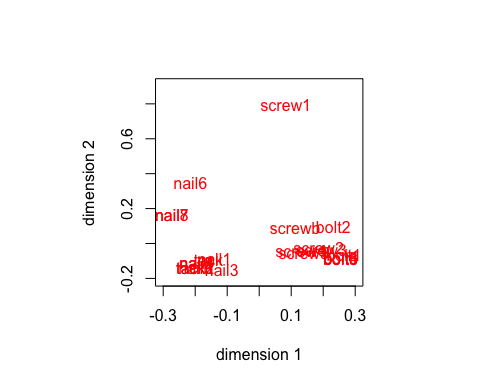
\includegraphics[keepaspectratio]{mca_files/figure-pdf/plot_hartigan_objscores-1.pdf}}
\end{center}

The star plots, produced by the utility \texttt{starPlotter()} are in
figure

\begin{center}
\pandocbounded{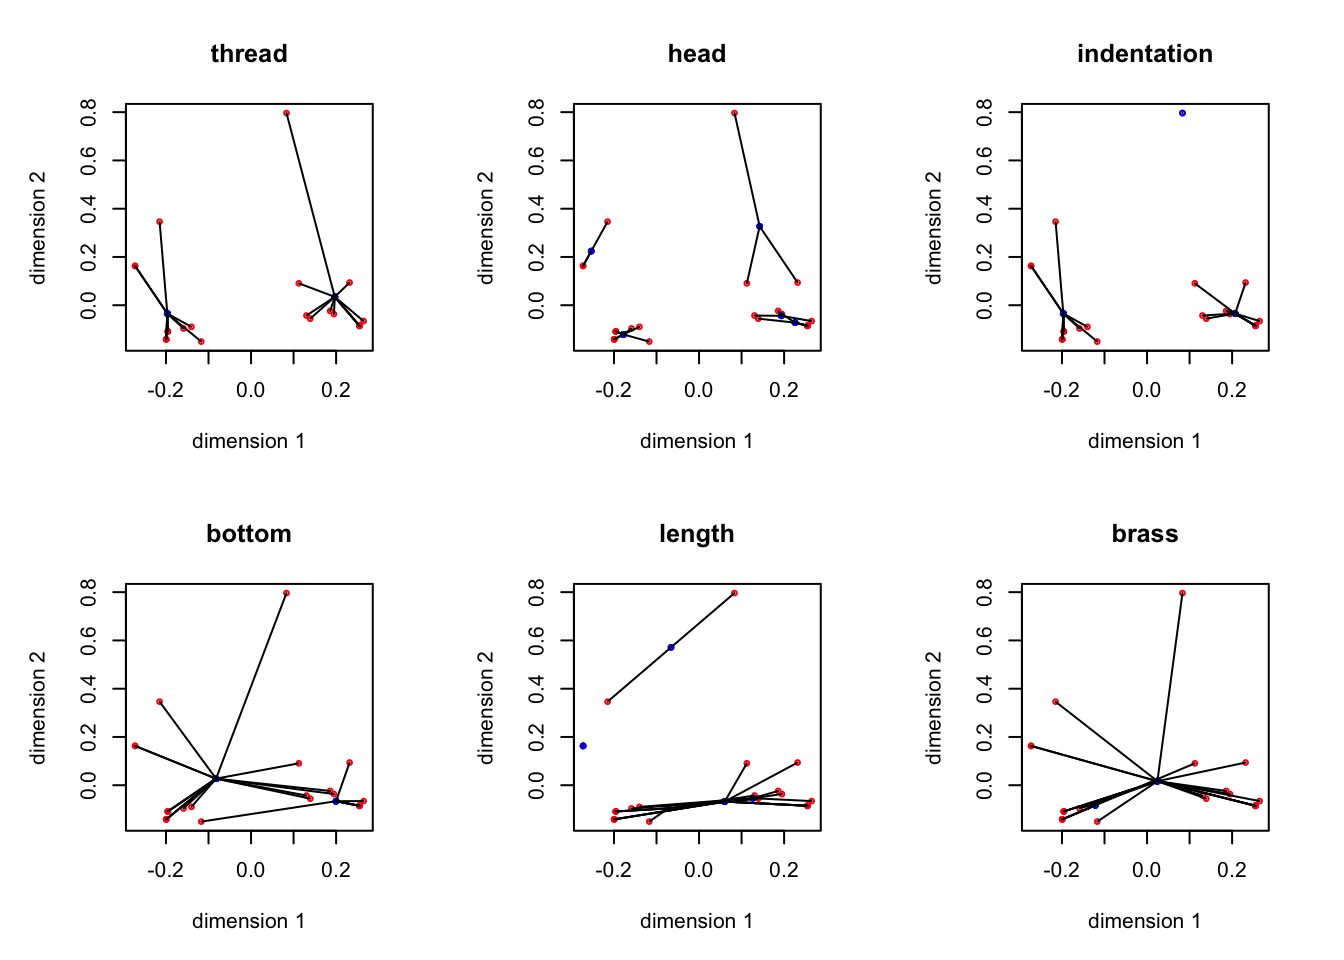
\includegraphics[keepaspectratio]{mca_files/figure-pdf/plot_hartigan_stars-1.pdf}}
\end{center}

The discriminations matrices \(\Delta_j\) are

\begin{verbatim}
     [,1]  [,2] 
[1,]  0.93  0.16
[2,]  0.16  0.03
     [,1]  [,2] 
[1,]  0.96  0.04
[2,]  0.04  0.64
     [,1]  [,2] 
[1,]  0.94  0.07
[2,]  0.07  0.66
     [,1]  [,2] 
[1,]  0.39 -0.13
[2,] -0.13  0.04
     [,1]  [,2] 
[1,]  0.29 -0.19
[2,] -0.19  0.82
     [,1]  [,2] 
[1,]  0.07  0.05
[2,]  0.05  0.03
\end{verbatim}

and their average \(\Lambda\) is

\begin{verbatim}
     [,1]  [,2] 
[1,]  0.60  0.00
[2,]  0.00  0.37
\end{verbatim}

Note that the loss was 0.5157273, which is one minus the average of the
trace of \(\Lambda\). The induced correlations are

\begin{verbatim}
      [,1]  [,2]  [,3]  [,4]  [,5]  [,6]  [,7]  [,8]  [,9] 
 [1,]  1.00  1.00  0.01  0.98 -0.20  0.46  0.03  0.41 -0.22
 [2,]  1.00  1.00  0.00  0.98 -0.21  0.46  0.03  0.41 -0.22
 [3,]  0.01  0.00  1.00  0.08  0.38  0.18 -0.59  0.40 -0.02
 [4,]  0.98  0.98  0.08  1.00 -0.00  0.50 -0.10  0.43 -0.21
 [5,] -0.20 -0.21  0.38 -0.00  1.00  0.14 -0.66  0.05  0.09
 [6,]  0.46  0.46  0.18  0.50  0.14  1.00 -0.17  0.28 -0.29
 [7,]  0.03  0.03 -0.59 -0.10 -0.66 -0.17  1.00 -0.00 -0.10
 [8,]  0.41  0.41  0.40  0.43  0.05  0.28 -0.00  1.00  0.23
 [9,] -0.22 -0.22 -0.02 -0.21  0.09 -0.29 -0.10  0.23  1.00
\end{verbatim}

Of the six variables, three are binary. Thus they only have a single
transformed variable associated with them, which is just the
standardization to mean zero and sum of squares one. The total number of
transformed variables is consequently 9. The eigenvalues of the induced
correlation matrix (divided by the number of variables, not the number
of transformed variables) are

\begin{verbatim}
[1]  0.60  0.37  0.21  0.13  0.10  0.07  0.02  0.00  0.00
\end{verbatim}

Note that the two dominant eigenvalues are again equal to the diagonal
elements of \(\Lambda\).

\#\#\#GALO

The second example is somewhat more realistic. In the GALO dataset
(Peschar (\citeproc{ref-peschar_75}{1975})) data on 1290 school children
in the sixth grade of an elementary school in 1959 in the city of
Groningen (Netherlands) were collected. The variables are gender, IQ
(categorized into 9 ordered categories), advice (teacher categorized the
children into 7 possible forms of secondary education, i.e., Agr =
agricultural; Ext = extended primary education; Gen = general; Grls =
secondary school for girls; Man = manual, including housekeeping; None =
no further education; Uni = pre- University), SES (parent's profession
in 6 categories) and school (37 different schools). The data have been
analyzed previously in many Gifi publications, for example in De Leeuw
and Mair (\citeproc{ref-deleeuw_mair_A_09a}{2009}). For our MCA we only
make the first four variables, school is treated as passive

We use this example to illustrate some of the constraints on
transformations. Two copies are used for all variables (although gender
effectively only has one, of course). IQ is treated as ordinal, using a
piecewise linear spline with knots at the nine data points.

\begin{Shaded}
\begin{Highlighting}[]
\NormalTok{galo\_knots }\OtherTok{\textless{}{-}} \FunctionTok{knotsD}\NormalTok{(galo)}
\NormalTok{galo\_degrees }\OtherTok{\textless{}{-}} \FunctionTok{c}\NormalTok{(}\SpecialCharTok{{-}}\DecValTok{1}\NormalTok{,}\DecValTok{1}\NormalTok{,}\SpecialCharTok{{-}}\DecValTok{1}\NormalTok{,}\SpecialCharTok{{-}}\DecValTok{1}\NormalTok{,}\SpecialCharTok{{-}}\DecValTok{1}\NormalTok{)}
\NormalTok{galo\_ordinal }\OtherTok{\textless{}{-}} \FunctionTok{c}\NormalTok{(}\ConstantTok{FALSE}\NormalTok{, }\ConstantTok{TRUE}\NormalTok{, }\ConstantTok{FALSE}\NormalTok{, }\ConstantTok{FALSE}\NormalTok{,}\ConstantTok{FALSE}\NormalTok{)}
\NormalTok{galo\_active }\OtherTok{\textless{}{-}}\FunctionTok{c}\NormalTok{ (}\ConstantTok{TRUE}\NormalTok{, }\ConstantTok{TRUE}\NormalTok{, }\ConstantTok{TRUE}\NormalTok{, }\ConstantTok{TRUE}\NormalTok{, }\ConstantTok{FALSE}\NormalTok{)}
\end{Highlighting}
\end{Shaded}

\begin{Shaded}
\begin{Highlighting}[]
\NormalTok{h }\OtherTok{\textless{}{-}} \FunctionTok{homals}\NormalTok{ (galo, }\AttributeTok{knots =}\NormalTok{ galo\_knots, }\AttributeTok{degrees =}\NormalTok{ galo\_degrees, }\AttributeTok{ordinal =}\NormalTok{ galo\_ordinal, }\AttributeTok{active =}\NormalTok{ galo\_active)}
\end{Highlighting}
\end{Shaded}

We first give transformations for the active variables (and their
copies) in figure . We skip gender, because transformation plots for
binary variables are not very informative. We give two transformation
plots for IQ, first using \(H\) and then using \(HA\). This illustrates
the point made earlier, that transformation plots of block scores for
ordinal variables with copies need not be monotone. It also illustrates
that additional copies of an ordinal variable are not scaled to be
monotone. Note that the plots for advice and SES are made with the
utility \texttt{stepPlotter()}. Because the degree of the splines for
those variables is zero, these transformation plots show step functions,
with the steps at the knots, which are represented by vertical lines.

\begin{center}
\pandocbounded{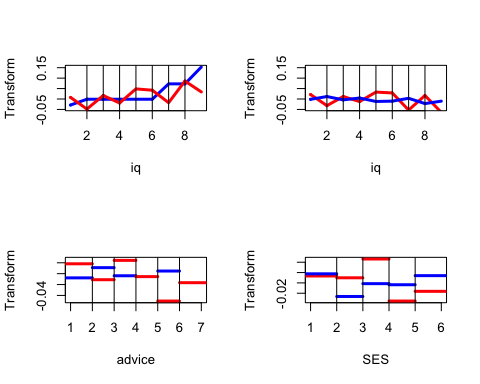
\includegraphics[keepaspectratio]{mca_files/figure-pdf/galo_trans-1.pdf}}
\end{center}

The four star plots for the active variables, together with the four
category quantification plots, are in figure . Note that
\texttt{homals()} does not compute category quantifications, we have to
compute them from the \texttt{homals()} output. Also note that for
gender, advice and SES the object scores are connected to the category
centroids of the variables. For IQ object scores are connected to points
on the line connecting adjacent category quantifications. See De Leeuw
and Rijckevorsel (\citeproc{ref-deleeuw_vanrijckevorsel_C_88}{1988}) for
category plots using forms of fuzzy coding (of which B-splines are an
example).

\begin{center}
\pandocbounded{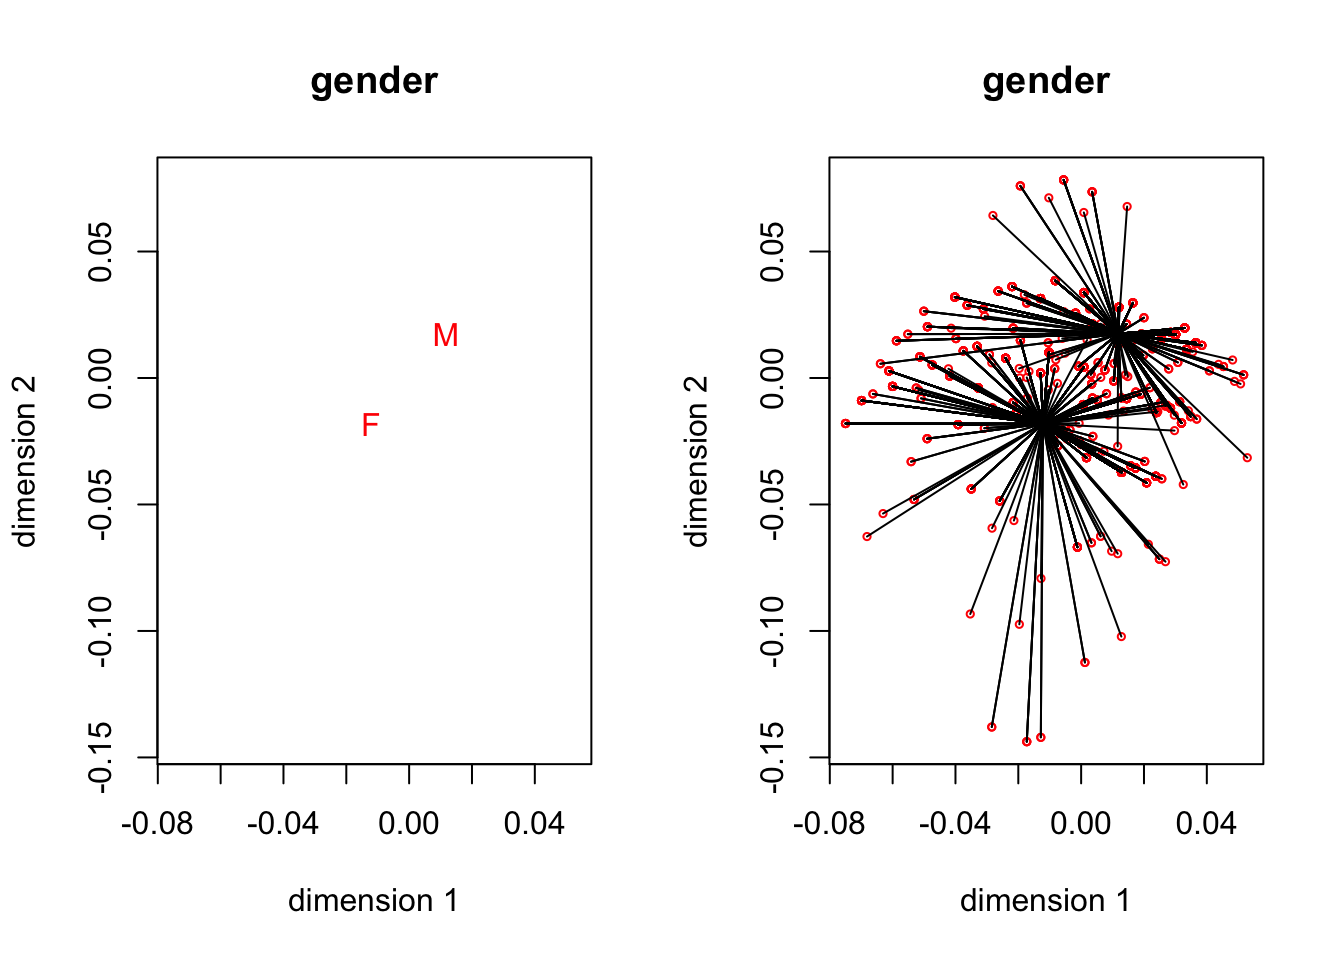
\includegraphics[keepaspectratio]{mca_files/figure-pdf/plot_galo_quant_stars-1.pdf}}
\end{center}

\begin{center}
\pandocbounded{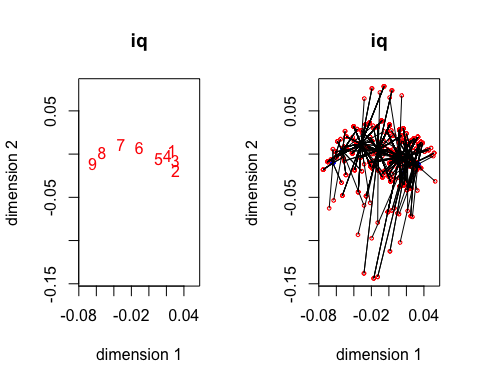
\includegraphics[keepaspectratio]{mca_files/figure-pdf/plot_galo_quant_stars-2.pdf}}
\end{center}

\begin{center}
\pandocbounded{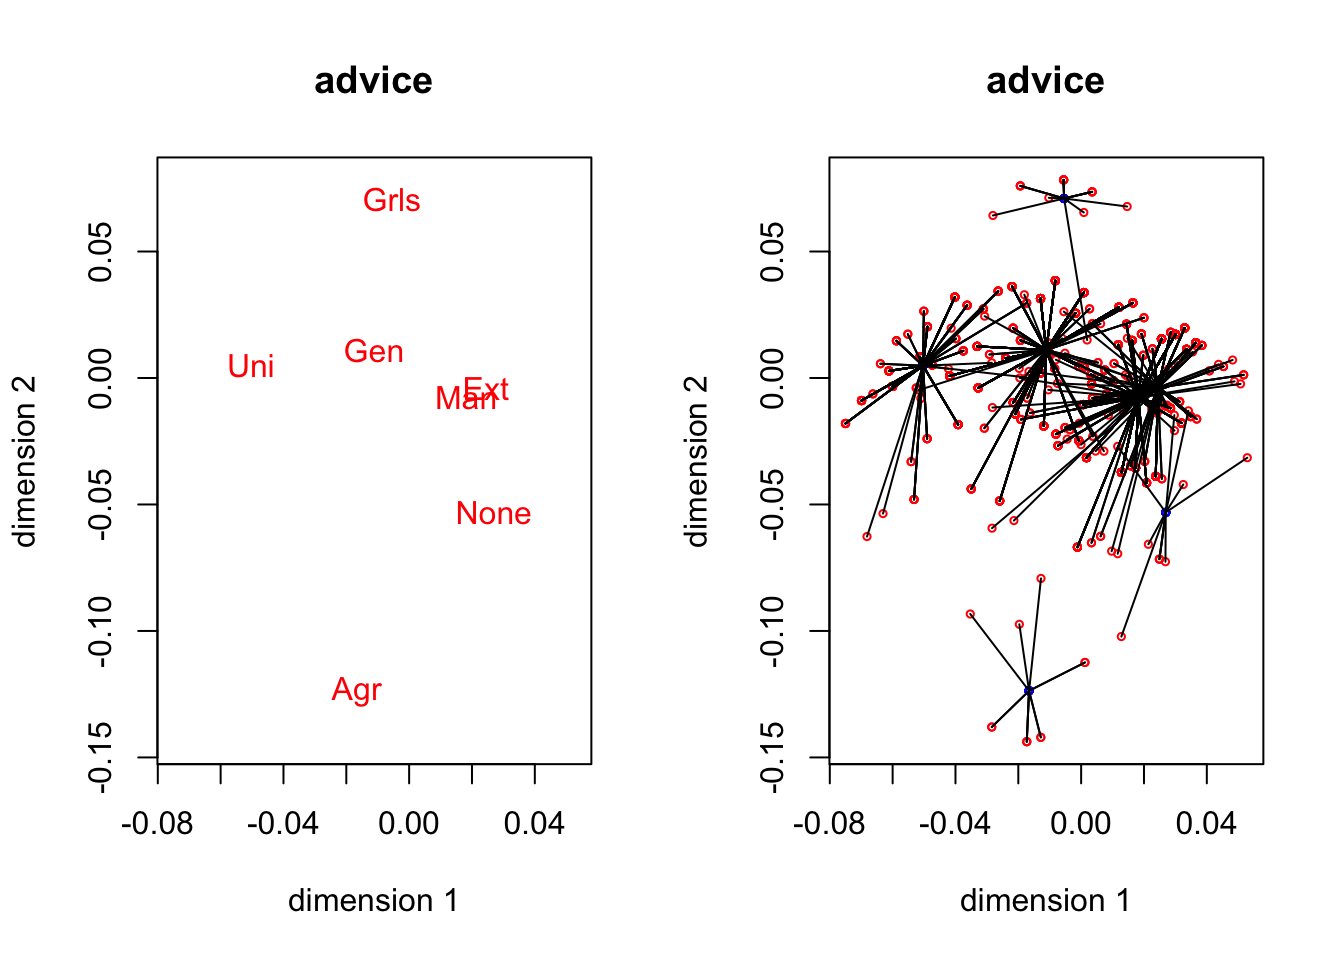
\includegraphics[keepaspectratio]{mca_files/figure-pdf/plot_galo_quant_stars-3.pdf}}
\end{center}

\begin{center}
\pandocbounded{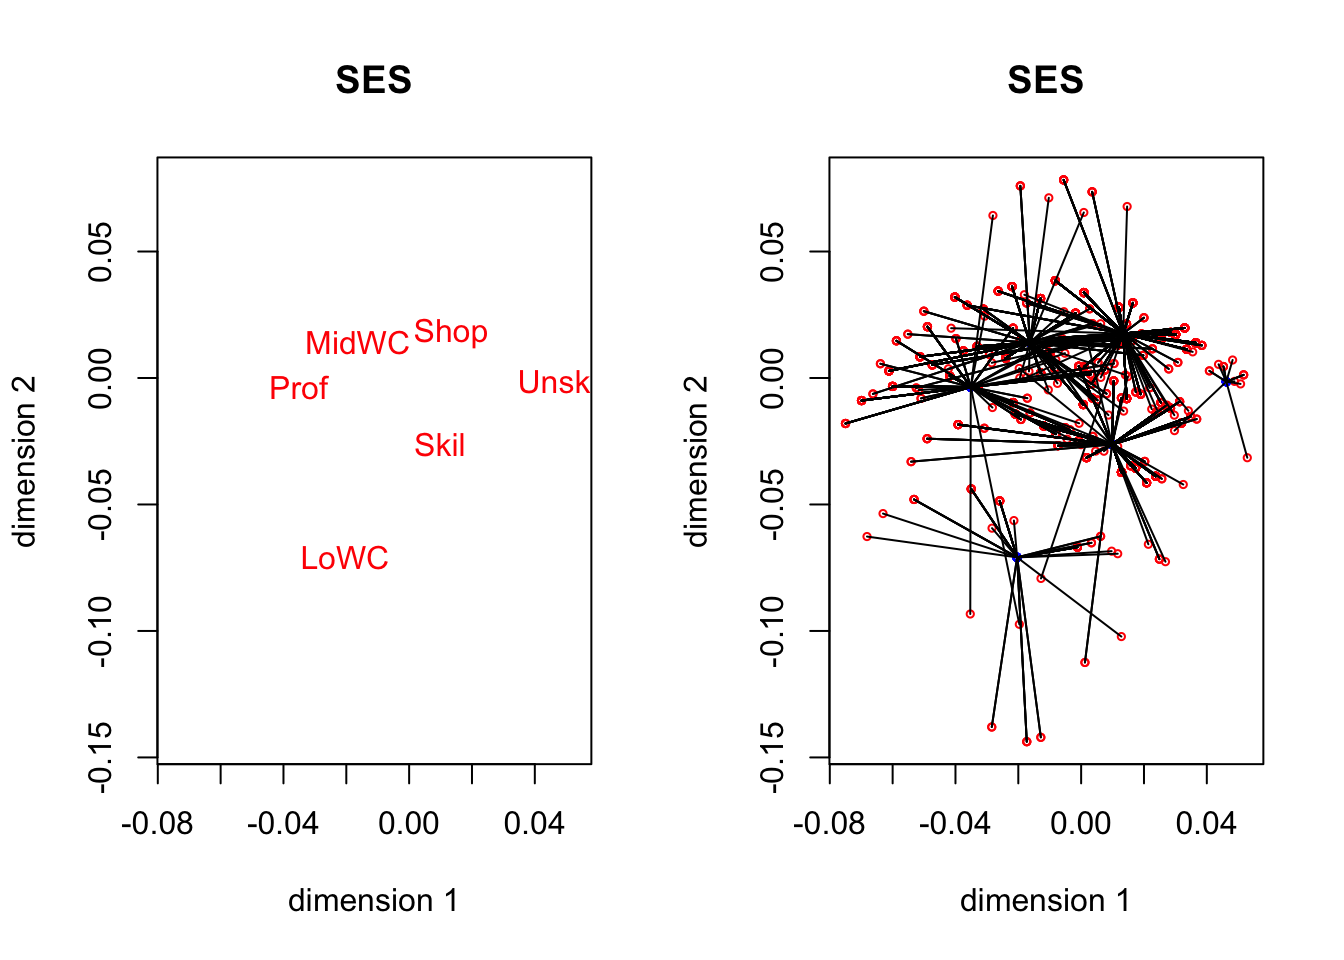
\includegraphics[keepaspectratio]{mca_files/figure-pdf/plot_galo_quant_stars-4.pdf}}
\end{center}

For this analysis we need 52 iterations to obtain loss 0.54251. The
average discrimination matrix over the four active variables is

\begin{verbatim}
     [,1]  [,2] 
[1,]  0.54  0.00
[2,]  0.00  0.38
\end{verbatim}

while the eigenvalues of the induced correlation matrix of the active
variables and their copies, divided by four, are

\begin{verbatim}
[1]  0.54  0.38  0.26  0.21  0.18  0.13  0.05
\end{verbatim}

The category quantifications for the passive variable indicating the 37
schools are in figure

\begin{center}
\pandocbounded{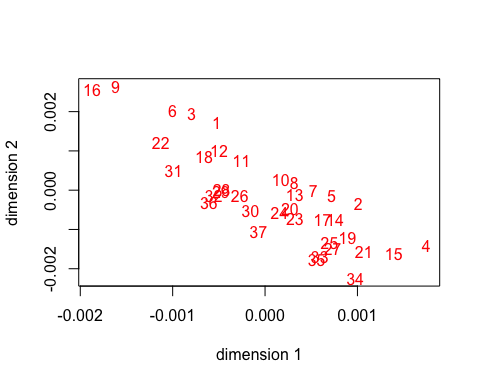
\includegraphics[keepaspectratio]{mca_files/figure-pdf/galo_school_passive_plot-1.pdf}}
\end{center}

If we look at the scale of the plot we see all schools are pretty close
to the origin. The discrimination matrices are consequently also small.
In 1959 schools were pretty much the same.

\begin{verbatim}
     [,1]    [,2]   
[1,]  0.0011 -0.0014
[2,] -0.0014  0.0022
\end{verbatim}

\subsection{Thirteen Personality
Scales}\label{thirteen-personality-scales}

Our next example is a small data block from the \texttt{psych} package
(\citeproc{ref-revelle_15}{Revelle 2015}) of five scales from the
Eysenck Personality Inventory, five from a Big Five inventory, a Beck
Depression Inventory, and State and Trait Anxiety measures.

\begin{Shaded}
\begin{Highlighting}[]
\NormalTok{epi}\OtherTok{\textless{}{-}} \FunctionTok{read.csv}\NormalTok{(}\StringTok{"data/epi.bfi.csv"}\NormalTok{)}
\NormalTok{epi\_knots }\OtherTok{\textless{}{-}} \FunctionTok{knotsQ}\NormalTok{(epi)}
\NormalTok{epi\_degrees }\OtherTok{\textless{}{-}} \FunctionTok{rep}\NormalTok{ (}\DecValTok{0}\NormalTok{, }\DecValTok{13}\NormalTok{)}
\NormalTok{epi\_ordinal }\OtherTok{\textless{}{-}} \FunctionTok{rep}\NormalTok{ (}\ConstantTok{FALSE}\NormalTok{, }\DecValTok{13}\NormalTok{)}
\end{Highlighting}
\end{Shaded}

We perform a two-dimensional MCA, using degree zero and inner knots at
the three quartiles for all 13 variables.

\begin{Shaded}
\begin{Highlighting}[]
\NormalTok{h }\OtherTok{\textless{}{-}} \FunctionTok{homals}\NormalTok{(epi, }\AttributeTok{knots =}\NormalTok{ epi\_knots, }\AttributeTok{degrees =}\NormalTok{ epi\_degrees, }\AttributeTok{ordinal =}\NormalTok{ epi\_ordinal)}
\end{Highlighting}
\end{Shaded}

We have convergence in 271 iterations to loss 0.7472906. The object
scores are in figure

\begin{center}
\pandocbounded{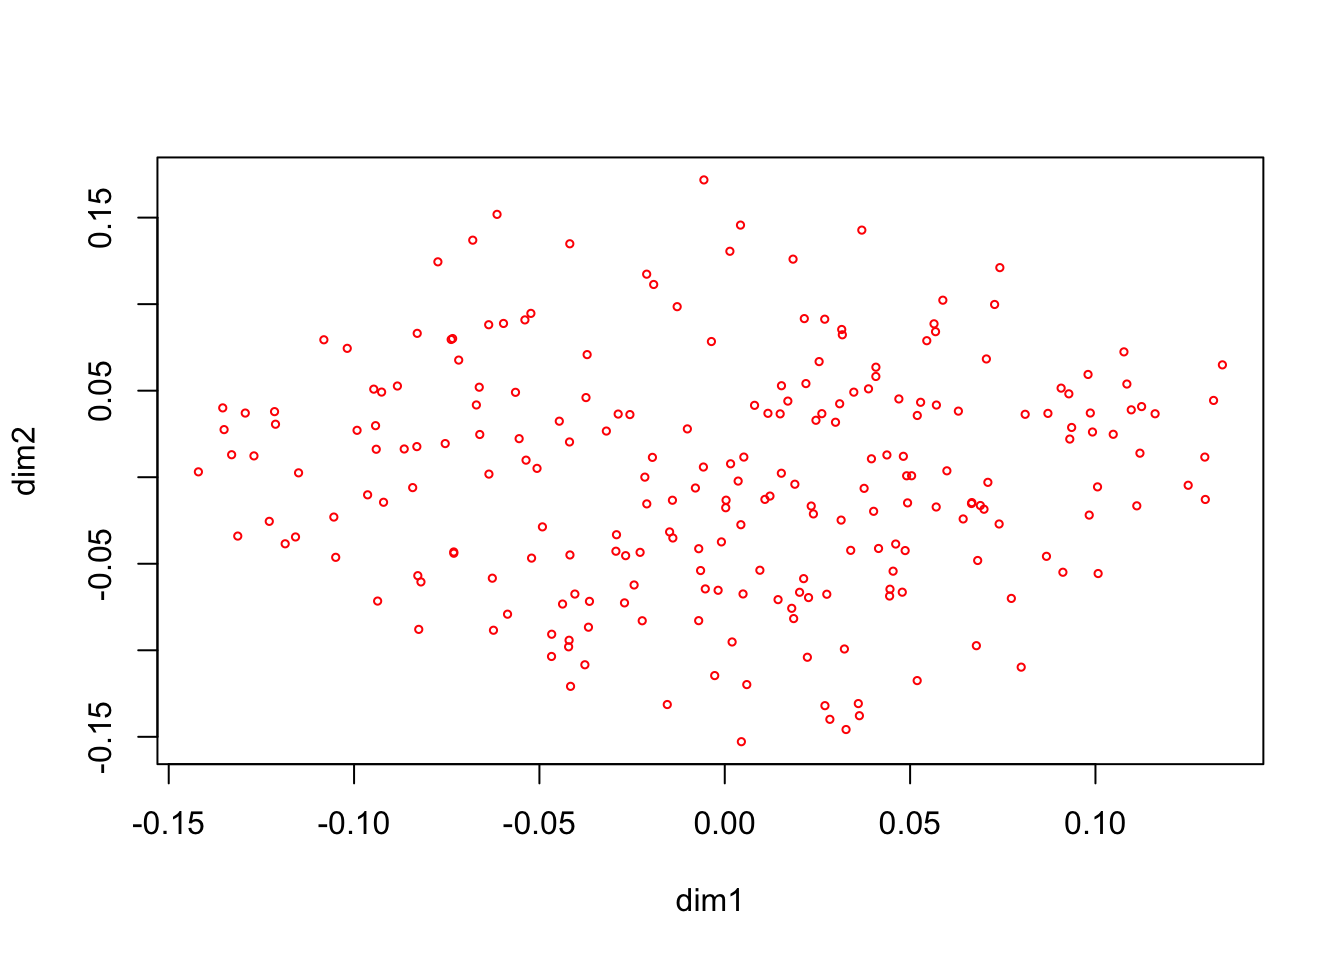
\includegraphics[keepaspectratio]{mca_files/figure-pdf/plot_epi_x_0-1.pdf}}
\end{center}

\begin{center}
\pandocbounded{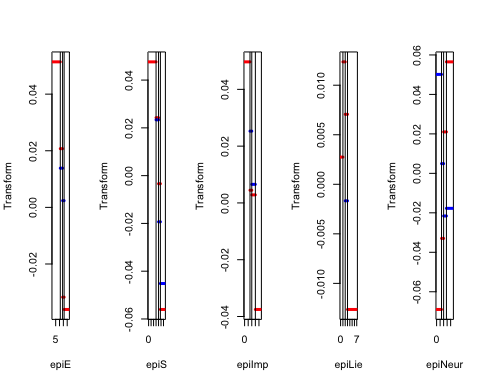
\includegraphics[keepaspectratio]{mca_files/figure-pdf/plot_epi_trans_0-1.pdf}}
\end{center}

\begin{center}
\pandocbounded{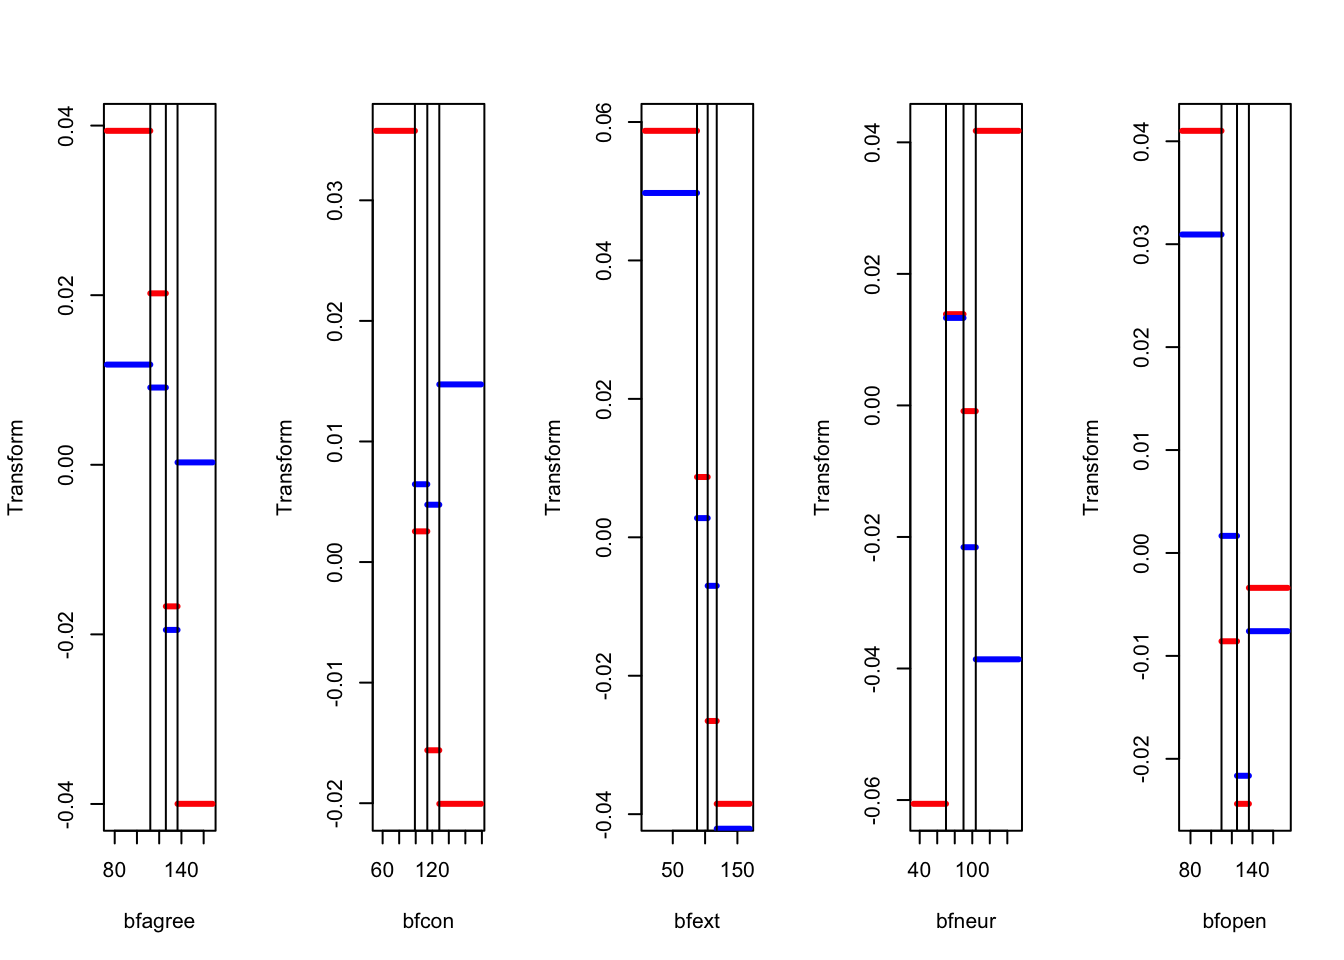
\includegraphics[keepaspectratio]{mca_files/figure-pdf/plot_epi_trans_0-2.pdf}}
\end{center}

\begin{center}
\pandocbounded{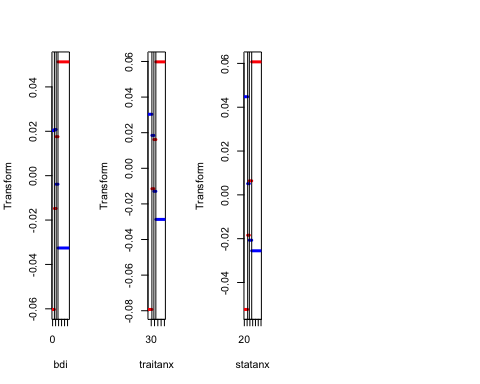
\includegraphics[keepaspectratio]{mca_files/figure-pdf/plot_epi_trans_0-3.pdf}}
\end{center}

The thirteen star plots are in figure

\begin{center}
\pandocbounded{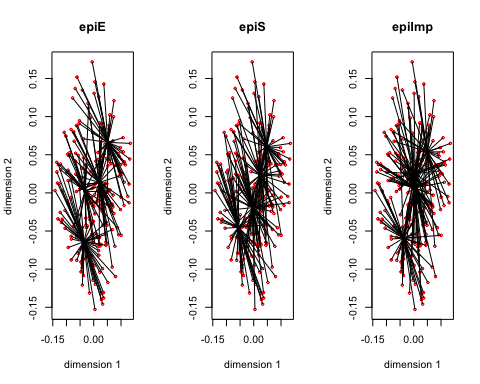
\includegraphics[keepaspectratio]{mca_files/figure-pdf/plot_epi_star_0-1.pdf}}
\end{center}

\begin{center}
\pandocbounded{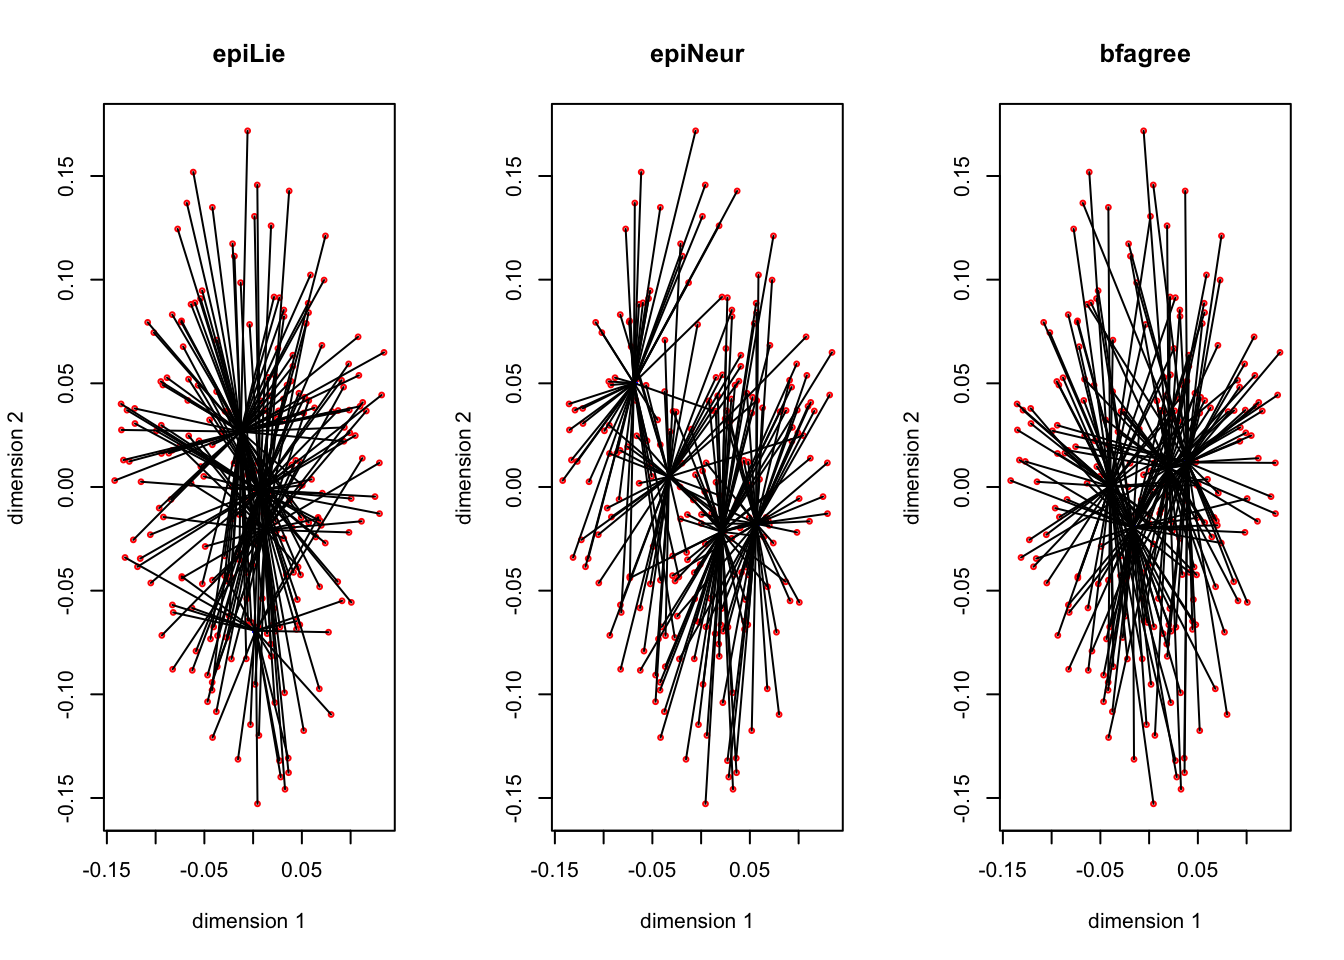
\includegraphics[keepaspectratio]{mca_files/figure-pdf/plot_epi_star_0-2.pdf}}
\end{center}

\begin{center}
\pandocbounded{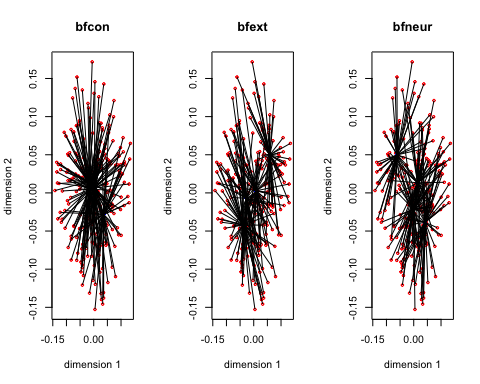
\includegraphics[keepaspectratio]{mca_files/figure-pdf/plot_epi_star_0-3.pdf}}
\end{center}

\begin{center}
\pandocbounded{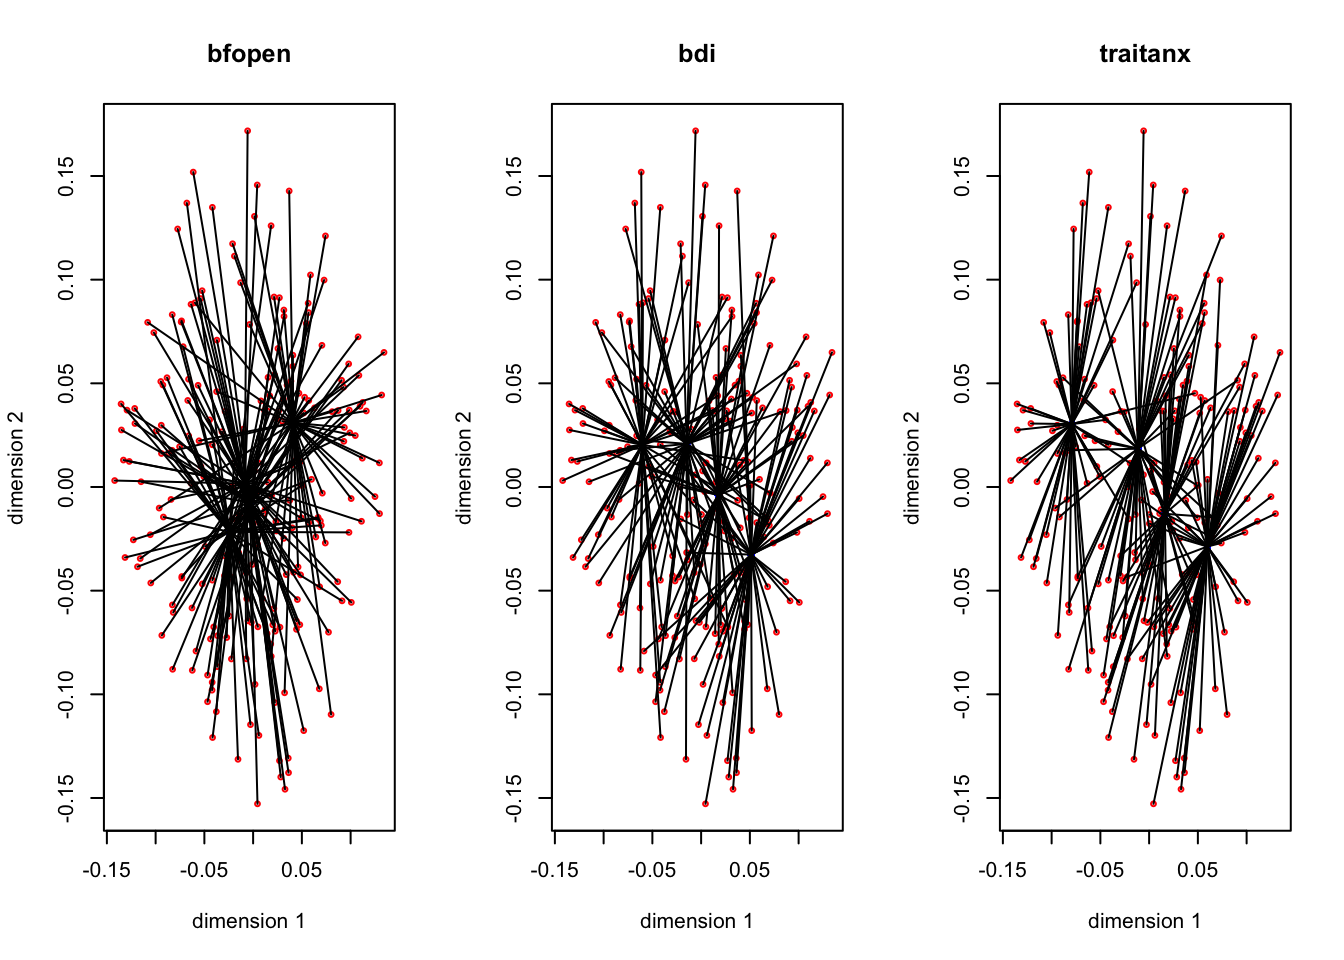
\includegraphics[keepaspectratio]{mca_files/figure-pdf/plot_epi_star_0-4.pdf}}
\end{center}

\begin{center}
\pandocbounded{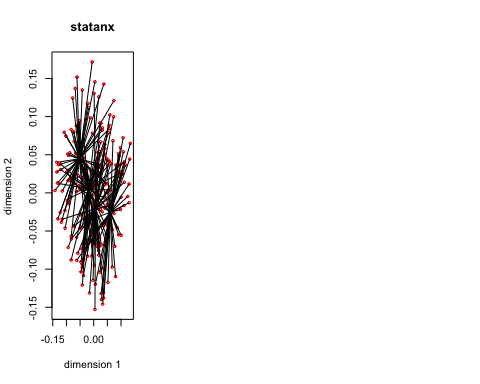
\includegraphics[keepaspectratio]{mca_files/figure-pdf/plot_epi_star_0-5.pdf}}
\end{center}

Now change the degree to two for all variables, i.e.~fit piecewise
quadratic polynomials which are differentiable at the knots. We still
have two copies for each variable, and these two copies define the
blocks.

\begin{Shaded}
\begin{Highlighting}[]
\NormalTok{epi\_degrees }\OtherTok{\textless{}{-}} \FunctionTok{rep}\NormalTok{ (}\DecValTok{2}\NormalTok{, }\DecValTok{13}\NormalTok{)}
\NormalTok{h }\OtherTok{\textless{}{-}} \FunctionTok{homals}\NormalTok{ (epi, }\AttributeTok{knots =}\NormalTok{ epi\_knots, }\AttributeTok{degrees =}\NormalTok{ epi\_degrees, }\AttributeTok{ordinal =}\NormalTok{ epi\_ordinal)}
\end{Highlighting}
\end{Shaded}

\begin{center}
\pandocbounded{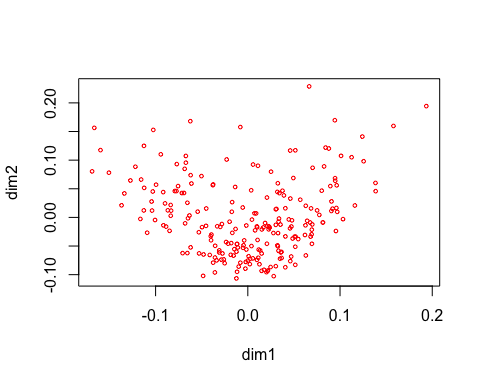
\includegraphics[keepaspectratio]{mca_files/figure-pdf/plot_epi_x_2-1.pdf}}
\end{center}

\begin{center}
\pandocbounded{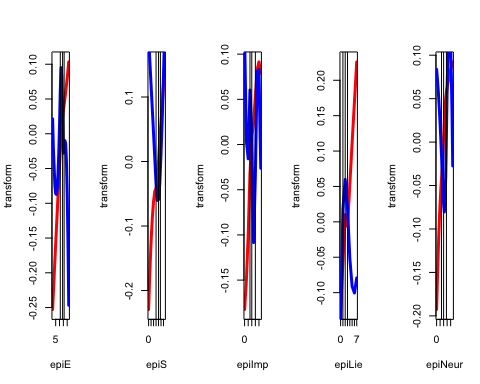
\includegraphics[keepaspectratio]{mca_files/figure-pdf/plot_epi_trans_2-1.pdf}}
\end{center}

\begin{center}
\pandocbounded{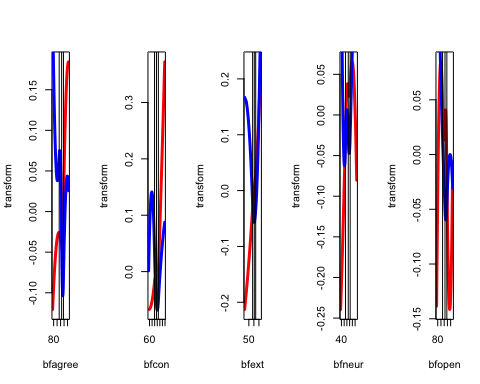
\includegraphics[keepaspectratio]{mca_files/figure-pdf/plot_epi_trans_2-2.pdf}}
\end{center}

\begin{center}
\pandocbounded{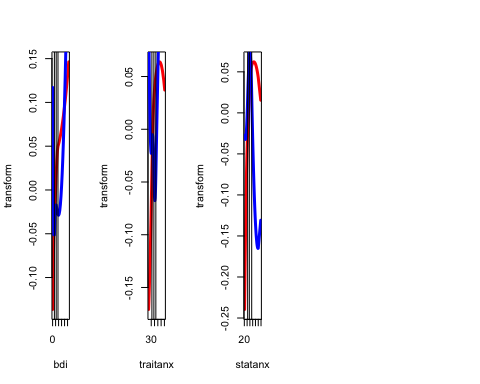
\includegraphics[keepaspectratio]{mca_files/figure-pdf/plot_epi_trans_2-3.pdf}}
\end{center}

\bookmarksetup{startatroot}

\chapter*{References}\label{references}
\addcontentsline{toc}{chapter}{References}

\markboth{References}{References}

\phantomsection\label{refs}
\begin{CSLReferences}{1}{0}
\bibitem[\citeproctext]{ref-bijleveld_deleeuw_A_91}
Bijleveld, C. C. J. H., and J. De Leeuw. 1991. {``{Fitting Longitudinal
Reduced-Rank Regression Models by Alternating Least Squares}.''}
\emph{Psychometrika} 56 (3): 433--47.

\bibitem[\citeproctext]{ref-bock_60}
Bock, R. D. 1960. {``{Methods and Applications of Optimal Scaling}.''}
Psychometric Laboratory Report 25. Chapell Hill, N.C.: L.L. Thurstone
Psychometric Laboratory, University of North Carolina.

\bibitem[\citeproctext]{ref-breiman_friedman_85}
Breiman, L., and J. H. Friedman. 1985. {``{Estimating Optimal
Transformations for Multiple Regression and Correlation}.''}
\emph{Journal of the American Statistical Association} 80: 580--619.

\bibitem[\citeproctext]{ref-vanderburg_deleeuw_verdegaal_A_88}
Burg, E. Van der, J. De Leeuw, and R. Verdegaal. 1988. {``Homogeneity
Analysis with {K} Sets of Variables: An Alternating Least Squares
Approach with Optimal Scaling Features.''} \emph{Psychometrika} 53:
177--97.

\bibitem[\citeproctext]{ref-carroll_68}
Carroll, J. D. 1968. {``{A Generalization of Canonical Correlation
Analysis to Three or More Sets of Variables}.''} In \emph{Proceedings of
the 76th Annual Convention of the American Psychological Association},
227--28. Washington, D.C.: American Psychological Association.

\bibitem[\citeproctext]{ref-coolen_deleeuw_R_87}
Coolen, H., and J. De Leeuw. 1987. {``{Least Squares Path Analysis with
Optimal Scaling}.''} Research Report RR-87-03. Leiden, The Netherlands:
Department of Data Theory FSW/RUL.

\bibitem[\citeproctext]{ref-cordier_65}
Cordier, B. 1965. {``{L'Analyse Factorielle des Correspondances}.''}
\{Th\textbackslash`ese de Troisieme Cycle\}, Université de Rennes.

\bibitem[\citeproctext]{ref-deleeuw_R_68e}
De Leeuw, J. 1968a. {``Canonical Discriminant Analysis of Relational
Data.''} Research Note 007-68. Department of Data Theory FSW/RUL.
\url{https://jansweb.netlify.app/publication/deleeuw-r-68-e/deleeuw-r-68-e.pdf}.

\bibitem[\citeproctext]{ref-deleeuw_R_68d}
---------. 1968b. {``Nonmetric Discriminant Analysis.''} Research Note
06-68. Department of Data Theory, University of Leiden.

\bibitem[\citeproctext]{ref-deleeuw_B_74}
---------. 1974. \emph{Canonical Analysis of Categorical Data}. Leiden,
The Netherlands: Psychological Institute, Leiden University.

\bibitem[\citeproctext]{ref-deleeuw_U_75a}
---------. 1975. {``{A Normalized Cone Regression Approach to
Alternating Least Squares Algorithms}.''} Department of Data Theory
FSW/RUL.
\url{https://jansweb.netlify.app/publication/deleeuw-u-75-a/deleeuw-u-75-a.pdf}.

\bibitem[\citeproctext]{ref-deleeuw_A_83b}
---------. 1983. {``On the Prehistory of Correspondence Analysis.''}
\emph{Statistica Neerlandica} 37: 161--64.

\bibitem[\citeproctext]{ref-deleeuw_C_84c}
---------. 1984. {``The Gifi System of Nonlinear Multivariate
Analysis.''} In \emph{Data Analysis and Informatics}, edited by E. Diday
et al. Vol. III. Amsterdam: North Holland Publishing Company.

\bibitem[\citeproctext]{ref-deleeuw_C_88b}
---------. 1988. {``{Multivariate Analysis with Optimal Scaling}.''} In
\emph{Proceedings of the International Conference on Advances in
Multivariate Statistical Analysis}, edited by S. Das Gupta and J. K.
Ghosh, 127--60. Calcutta, India: Indian Statistical Institute.

\bibitem[\citeproctext]{ref-deleeuw_C_94c}
---------. 1994. {``{Block Relaxation Algorithms in Statistics}.''} In
\emph{Information Systems and Data Analysis}, edited by H. H. Bock, W.
Lenski, and M. M. Richter, 308--24. Berlin: Springer Verlag.
\url{https://jansweb.netlify.app/publication/deleeuw-c-94-c/deleeuw-c-94-c.pdf}.

\bibitem[\citeproctext]{ref-deleeuw_C_04a}
---------. 2004. {``Least Squares Optimal Scaling of Partially Observed
Linear Systems.''} In \emph{Recent Developments in Structural Equation
Models}, edited by K. van Montfort, J. Oud, and A. Satorra. Dordrecht,
Netherlands: Kluwer Academic Publishers.

\bibitem[\citeproctext]{ref-deleeuw_R_09c}
---------. 2009. {``{Regression, Discriminant Analysis, and Canonical
Analysis with homals}.''} Preprint Series 562. Los Angeles, CA: UCLA
Department of Statistics.

\bibitem[\citeproctext]{ref-deleeuw_E_15b}
---------. 2015a. {``{Aspects of Correlation Matrices}.''}
\url{https://jansweb.netlify.app/publication/deleeuw-e-15-b/deleeuw-e-15-b.pdf}.

\bibitem[\citeproctext]{ref-deleeuw_E_15d}
---------. 2015b. {``Exceedingly Simple b-Spline Code.''}

\bibitem[\citeproctext]{ref-deleeuw_E_15e}
---------. 2015c. {``Regression with Linear Inequality Restrictions on
Predicted Values.''}

\bibitem[\citeproctext]{ref-deleeuw_mair_A_09a}
De Leeuw, J., and P. Mair. 2009. {``{Homogeneity Analysis in {R}: the
Package homals}.''} \emph{Journal of Statistical Software} 31 (4):
1--21. \url{https://www.jstatsoft.org/v31/i04/}.

\bibitem[\citeproctext]{ref-deleeuw_vanrijckevorsel_C_80}
De Leeuw, J., and J. L. A. Van Rijckevorsel. 1980. {``{HOMALS} and
{PRINCALS}: Some Generalizations of Principal Components Analysis.''} In
\emph{Data Analysis and Informatics}. Amsterdam: North Holland
Publishing Company.

\bibitem[\citeproctext]{ref-deleeuw_vanrijckevorsel_C_88}
---------. 1988. {``Beyond Homogeneity Analysis.''} In \emph{Component
and Correspondence Analysis}, edited by J. L. A. Van Rijckevorsel and J.
De Leeuw, 55--80. Chichester, England: Wiley.

\bibitem[\citeproctext]{ref-deleeuw_vanrijckevorsel_vanderwouden_A_81}
De Leeuw, J., J. L. A. Van Rijckevorsel, and H. Van der Wouden. 1981.
{``Nonlinear Principal Component Analysis Using b-Splines.''}
\emph{Methods of Operations Research} 43: 379--94.

\bibitem[\citeproctext]{ref-gibson_62}
Gibson, W. A. 1962. {``{On the Least Squares Orthogonalization of an
Oblique Transformation}.''} \emph{Psychometrika} 27: 193--95.

\bibitem[\citeproctext]{ref-gifi_B_80}
Gifi, A. 1980. \emph{Niet-Lineaire Multivariate Analyse {[}Nonlinear
Multivariate Analysis{]}}. Leiden, The Netherlands: Department of Data
Theory FSW/RUL.

\bibitem[\citeproctext]{ref-gifi_B_81}
---------. 1981. \emph{Nonlinear Multivariate Analysis}. Leiden, The
Netherlands: Department of Data Theory FSW/RUL.

\bibitem[\citeproctext]{ref-gifi_B_90}
---------. 1990. \emph{Nonlinear Multivariate Analysis}. New York, N.Y.:
Wiley.

\bibitem[\citeproctext]{ref-gower_90}
Gower, J. C. 1990. {``{Fisher's Optimal Scores and Multiple
Correspondence Analysis}.''} \emph{Biometrics} 46: 947--61.

\bibitem[\citeproctext]{ref-gower_hand_96}
Gower, J. C., and D. J. Hand. 1996. \emph{{Biplots}}. Monographs on
Statistics and Applied Probability 54. {Chapman \& Hall}.

\bibitem[\citeproctext]{ref-gower_leroux_gardnerlubbe_15}
Gower, J. C., N. J. Le Roux, and S. Gardner-Lubbe. 2015. {``{Biplots:
Quantitative Data}.''} \emph{WIREs Computational Statistics} 7: 42--62.

\bibitem[\citeproctext]{ref-gower_leroux_gardnerlubbe_16}
---------. 2016. {``{Biplots: Qualitative Data}.''} \emph{WIREs
Computational Statistics} 8: 82--111.

\bibitem[\citeproctext]{ref-guttman_41}
Guttman, L. 1941. {``{The Quantification of a Class of Attributes: A
Theory and Method of Scale Construction}.''} In \emph{The Prediction of
Personal Adjustment}, edited by P. Horst, 321--48. New York: Social
Science Research Council.

\bibitem[\citeproctext]{ref-hartigan_75}
Hartigan, J. 1975. \emph{Clustering Algorithms}. Wiley.

\bibitem[\citeproctext]{ref-heiser_95}
Heiser, W. J. 1995. {``{Convergent Computing by Iterative Majorization:
Theory and Applications in Multidimensional Data Analysis}.''} In
\emph{Recent Advantages in Descriptive Multivariate Analysis}, edited by
W. J. Krzanowski, 157--89. Oxford: Clarendon Press.

\bibitem[\citeproctext]{ref-hill_74}
Hill, M. O. 1974. {``{Correspondence Analysis: a Neglected Multivariate
Method}.''} \emph{Applied Statistics} 23: 340--54.

\bibitem[\citeproctext]{ref-hill_90}
---------. 1990. {``{Review of A. Gifi, Multivariate Analysis}.''}
\emph{Journal of Ecology} 78 (4): 1148--49.

\bibitem[\citeproctext]{ref-holland_79}
Holland, P. W. 1979. {``{The Tyranny of Continuous Models in a World of
Discrete Data}.''} \emph{IHS-Journal} 3: 29--42.

\bibitem[\citeproctext]{ref-ibm_15}
IBM. 2015. \emph{IBM SPSS Categories 23}. IBM Corporation.

\bibitem[\citeproctext]{ref-koyak_87}
Koyak, R. 1987. {``{On Measuring Internal Dependence in a Set of Random
Variables}.''} \emph{Annals of Statistics} 15: 1215--28.

\bibitem[\citeproctext]{ref-kruskal_64a}
Kruskal, J. B. 1964a. {``{Multidimensional Scaling by Optimizing
Goodness of Fit to a Nonmetric Hypothesis}.''} \emph{Psychometrika} 29:
1--27.

\bibitem[\citeproctext]{ref-kruskal_64b}
---------. 1964b. {``{Nonmetric Multidimensional Scaling: a Numerical
Method}.''} \emph{Psychometrika} 29: 115--29.

\bibitem[\citeproctext]{ref-kruskal_65}
---------. 1965. {``{Analysis of Factorial Experiments by Estimating
Monotone Transformations of the Data}.''} \emph{Journal of the Royal
Statistical Society} B27: 251--63.

\bibitem[\citeproctext]{ref-kruskal_shepard_74}
Kruskal, J. B., and R. N. Shepard. 1974. {``{A Nonmetric Variety of
Linear Factor Analysis}.''} \emph{Psychometrika} 39: 123--57.

\bibitem[\citeproctext]{ref-lange_hunter_yang_00}
Lange, K., D. R. Hunter, and I. Yang. 2000. {``{Optimization Transfer
Using Surrogate Objective Functions}.''} \emph{Journal of Computational
and Graphical Statistics} 9: 1--20.

\bibitem[\citeproctext]{ref-lingoes_73}
Lingoes, J. C. 1973. \emph{{The Guttman-Lingoes Nonmetric Program
Series}}. Mathesis Press.

\bibitem[\citeproctext]{ref-mair_deleeuw_A_10}
Mair, P., and J. De Leeuw. 2010. {``A General Framework for Multivariate
Analysis with Optimal Scaling: The r Package Aspect.''} \emph{Journal of
Statistical Software} 32 (9): 1--23.

\bibitem[\citeproctext]{ref-marvell_53}
Marvell, A. 1653. {``The Character of Holland.''}

\bibitem[\citeproctext]{ref-meulman_82}
Meulman, J. J. 1982. \emph{{Homogeneity Analysis of Incomplete Data}}.
Leiden, The Netherlands: {DSWO} Press.

\bibitem[\citeproctext]{ref-meulman_heiser_12}
Meulman, J. J., and W. J. Heiser. 2012. \emph{IBM SPSS Categories 21}.
IBM Corporation.

\bibitem[\citeproctext]{ref-michailidis_deleeuw_A_98}
Michailidis, G., and J. De Leeuw. 1998. {``The Gifi System for
Descriptive Multivariate Analysis.''} \emph{Statistical Science} 13:
307--36.

\bibitem[\citeproctext]{ref-peschar_75}
Peschar, J. L. 1975. \emph{{School, Milieu, Beroep}}. Groningen, The
Netherlands: Tjeek Willink.

\bibitem[\citeproctext]{ref-revelle_15}
Revelle, William. 2015. \emph{Psych: Procedures for Psychological,
Psychometric, and Personality Research}. Evanston, Illinois:
Northwestern University.

\bibitem[\citeproctext]{ref-roskam_68}
Roskam, E. E. 1968. {``{Metric Analysis of Ordinal Data in
Psychology}.''} PhD thesis, University of Leiden.

\bibitem[\citeproctext]{ref-spss_89}
SPSS. 1989. \emph{SPSS Categories}. SPSS Inc.

\bibitem[\citeproctext]{ref-takane_92}
Takane, Y. 1992. {``{Review of Albert Gifi, Nonlinear Multivariate
Analysis}.''} \emph{Journal of the American Statistical Association} 87:
587--88.

\bibitem[\citeproctext]{ref-tanaka_79}
Tanaka, Y. 1979. {``{Review of the Methods of Quantification}.''}
\emph{Environmental Health Perspectives} 32: 113--23.

\bibitem[\citeproctext]{ref-vanderheijden_vanbuuren_16}
Van der Heijden, P. G. M., and S. Van Buuren. 1916. {``Looking Back at
the Gifi System of Nonlinear Multivariate Analysis.''} \emph{Journal of
Statistical Software} 73 (4).

\bibitem[\citeproctext]{ref-vanrijckevorsel_deleeuw_B_88}
Van Rijckevorsel, J. L. A., and J. De Leeuw, eds. 1988. \emph{Component
and Correspondence Analysis}. Wiley.

\bibitem[\citeproctext]{ref-winsberg_ramsay_80}
Winsberg, S., and J. O. Ramsay. 1980. {``{Monotone Transformations to
Additivity}.''} \emph{Biometrika} 67: 669--74.

\bibitem[\citeproctext]{ref-winsberg_ramsay_83}
---------. 1983. {``{Monotone Spline Transformations for Dimension
Reduction}.''} \emph{Psychometrika} 48: 575--95.

\bibitem[\citeproctext]{ref-xie_15}
Xie, Y. 2015. \emph{{Dynamic Documents with R and knitr}}. Second
Edition. CRC Press.

\bibitem[\citeproctext]{ref-xie_16}
---------. 2016. \emph{Bookdown: Authoring Books with r Markdown.}

\bibitem[\citeproctext]{ref-young_81}
Young, F. W. 1981. {``{Quantitative Analysis of Qualitative Data}.''}
\emph{Psychometrika} 46: 357--88.

\bibitem[\citeproctext]{ref-young_deleeuw_takane_C_80}
Young, F. W., J. De Leeuw, and Y. Takane. 1980. {``Quantifying
Qualitative Data.''} In \emph{Similarity and Choice. Papers in Honor of
Clyde Coombs}, edited by E. D. Lantermann and H. Feger. Bern: Hans
Huber.

\end{CSLReferences}


\backmatter


\end{document}
